%% main file: 主控文件

% ======================= 导言区 ============================
\documentclass[12pt,oneside,openright]{book}

\usepackage{mxystyle}

% ======================= 部分调试 ============================
%\includeonly{parts/part1/p1c1-dynamic-macro}


% ======================= 开始 ============================
\begin{document}

% ===== 前辅文 =====
\frontmatter

\maketitle
% 封面、前言
%% Cover

\MakeLinkTarget*{cover}
\pdfbookmark{Cover}{cover}

% 封面内容
\cover
%%% Title Page

\pagestyle{empty}
\topskip0pt
\vspace*{20em}

\begin{center}
    {\bfseries\Huge 量化宏观经济学}
\end{center}

\newpage
%%% copyright

\thispagestyle{empty}
\topskip0pt
\vspace*{\fill}

\begin{center}
    \begin{tabular}{c}
        \textbf{量化宏观经济学} \\
        \\\\\\\\
        \textbf{Liu}，\textit{中国人民大学}；\\
        \\\\
        \textbf{满翔宇}, \textit{中国人民大学}
    \end{tabular}
\end{center}
\vspace*{\fill}
%%% preface

\thispagestyle{empty}
\MakeLinkTarget*{preface}

% 添加书签
\pdfbookmark{Preface}{preface}

% 格式
\topskip0pt

% 居中显示：Preface
\begin{center}
    {\bfseries\sffamily\Huge 前言}
\end{center}

% 内容
\vspace{4em}
前言

\vspace*{1em}
\hspace*{\fill}{\itshape 满翔宇}

\noindent \hspace{\fill}{\itshape 江苏~徐州}

\noindent \hspace{\fill}{\itshape 2025年6月}

% 目录
\tableofcontents
%%% Contents

\MakeLinkTarget*{contents}
\pdfbookmark{Contents}{contents}
\tableofcontents
\pagenumbering{arabic}
\setcounter{page}{0}


% ===== 主体内容 =====
\mainmatter

% 第一篇：量化宏观基础
\part{量化宏观基础}

% 第1章 索洛模型与序列视角下的动态优化

% 导言

\chapter{序列视角下的动态优化} \label{ch-dynamic-opt-sq}

现代宏观经济学通过优化经济主体行为来研究经济运行的动态运行过程。因此，动态优化是学习量化宏观的基础。
宏观经济理论发展至今，对动态优化问题形成了两种处理方法：
一是序列问题视角，通过求解差分（微分）方程为经济主体选择一个最优的序列（有限或是无穷），这是处理动态问题的基础视角；
二是递归视角：定义从当期到下期的映射，利用动态规划方法将优化问题转化为泛函方程的求解。

本章通过宏观经济学中两种重要模型对序列视角下的动态优化进行初步介绍：消费-储蓄模型和新古典增长模型。
借助消费-储蓄问题，我们将初步了解优化问题的序列求解方法。
接着，我们将详细学习新古典增长理论：先对经典的索洛模型进行回顾，深化对动态宏观基本概念和理论的认识；
然后，借助现代宏观经济学的基石模型（Workhouse Model）——新古典增长模型（或称最优增长模型），
深化对序列视角下动态优化理论的理解，为下一章递归方法和动态规划学习奠定基础。


% =============== main ch1 ===============

% 1.1 =============== 消费-储蓄模型 ===============

\section{动态优化引例：消费-储蓄问题} \label{sec-consumption-saving}



% 1.2 =============== 新古典理论 ===============

\section{新古典增长理论} \label{sec-ngm}

接下来，我们将通过另一个重要模型来深入对序列视角下动态优化问题的认知，这就是新古典增长模型（或称最优增长模型）。
新古典理论是在Solow等人的工作之上建立起来的。在当时，美国长期稳定的资本产出比引起了许多经济学家的关注。
早期增长理论如哈罗德-多马模型将这一特征直接作为模型的前提假设：资本与劳动必须按固定比例结合（互补）才能进行生产。
但是索罗发现，资本和劳动明显是可替代的，传统理论不能解释现实问题：
数据上看，劳动的价格（工资）趋势性上升，在生产要素互补的情形下，资本租金率也应当上升，这与观察到的稳定的资本租金率不符。

索洛认为，这些现象可以由\textbf{新古典}视角加以解释。如果一个生产函数关于其投入要素是\textbf{边际报酬递减的}，
我们通常称其具有\textbf{新古典特征}。在这一生产函数下，当人均资本提高，资本的边际产出会降低，在竞争市场上这会反应为要素价格的变化。
而如果同时存在劳动增进的技术进步，就可以解释特征事实中要素数量和价格的相关特征。由此，一个将新古典特征和技术进步相结合的理论诞生了。
Solow（1956）和Swan（1956）在Ramsey（1928）、哈罗德-多马模型等理论的基础上，建立了Solow-Swan模型，
奠定了新古典增长理论（Neoclassical Growth）和现代宏观经济学的基础。

在本节我们将重点介绍新古典增长模型的起源——索洛模型，并引出相关宏观经济学的概念。
我们将在下一节重点研究最优增长模型的序列化解法。


% 1.2.1 ===== 基准 =====
\subsection{基准索洛模型}

索洛模型的核心要素是\textbf{总量生产函数}（Aggregate Production Function），
通常由总资本$K_t$，总劳动投入$L_t$（人口乘人均工作时间）和技术$A_t$构成。
我们从最简单的情形开始来介绍相关概念。在这一模型中，没有技术进步或人口和工人技能特征，从而总量生产函数为：
\begin{equation*}
    Y_t = F\left(K_t, L_t\right)
\end{equation*}
其中$Y_t$可以理解为经济的GDP。对于函数$F(K, L)$，有如下假设：
\begin{assumption}  \label{as-F-increase}
    $F(K, L)$关于$k$和$L$严格递增
\end{assumption}
\begin{assumption}  \label{as-F-quasiconcave}
    $F(K, L)$关于$(K, L)$严格拟凹
\end{assumption}
\begin{assumption}  \label{as-F-cosntant}
    $F(K, L)$关于$(K, L)$规模报酬不变
\end{assumption}
\begin{assumption}  \label{as-F-zero}
    $F(0, L)=0$
\end{assumption}
\begin{assumption}  \label{as-F-inada}
    \textbf{Inada条件}：$\lim\limits_{K\rightarrow 0}F_1(K, L)
        = \infty, \quad \lim\limits_{K\rightarrow \infty}F_1(K, L)=0$
\end{assumption}

在基准模型中，假设人口总数$N_t$和人均工作时间$l_t$为常数，因此$L_t$为常数。
将人口总数和人均工时正则化为1，从而生产函数中剩下的变量只有$K_t$，结合规模报酬不变，可以写出人均形式：
\begin{equation*}
    F(K_t, 1)=F(k_t, 1)\equiv f(k_t)
\end{equation*}
我们以小写字母表示人均测度，生产函数可以表示为：
\begin{equation}
    y_t = f(k_t)
\end{equation}
索洛模型的另一个核心构成是\textbf{资本运动方程}：
\begin{equation}    
    k_{t+1} = i_t + (1-\delta)k_t
\end{equation}
其中$i_t$表示$t$期的（人均）投资，$\delta k_t$表示既有资本的折旧，$\delta\in (0,1)$表示折旧率。
索洛模型隐性地假定了产品的同质性，可被用于消费或投资,根据供给等于需求：
\begin{equation}
    y_t = c_t + i_t
\end{equation}
在索洛模型中，并没有对消费者的消费-储蓄问题建模，而是假设\textbf{外生储蓄率}$s\in(0,1)$。
由于$y_t$不仅是产品供给，同时也是消费者的总收入，即它不是被用于消费就是被用于储蓄，因此总投资等于总储蓄：
\begin{equation}
    i_t = s y_t
\end{equation}
从而我们可以得到\textbf{资本运动方程的差分形式}：
\begin{equation}    \label{eq-k-law-of-motion}
    k_{t+1} = (1-\delta)k_t + sf(k_t)
\end{equation}
这是索洛模型的核心方程：右侧唯一的内生变量是资本存量$k_t$，下期的内生资本水平仅由当期资本水平决定。
注意到，对于外生给定的$k_0$，我们可以由上式得到资本序列$\{k_{t+1}\}_{t=0}^{\infty}$，
进而同时也能得到人均产出、消费和投资（储蓄）。


% 1.2.2 ===== 稳态 =====
\subsection{稳态与动态}

对\cref{eq-k-law-of-motion}，考虑$k_t$不随时间变化这一特殊情形，我们称其为\textbf{稳态}，
记为$k_t=\bar{k},~\forall t$。它是如下方程的解：
\begin{equation*}
    \bar{k}=(1-\delta) \bar{k}+s f(\bar{k})
\end{equation*}
这表明在稳态时，$\delta \bar{k} = sf(\bar{k})$。方程左侧是一条通过原点的直线；
方程右侧是通过原点、严格递增并且严格凹的曲线，它在0处斜率趋近无穷，$\bar{k}\rightarrow \infty$时斜率趋近0。
这样的\textbf{Inada条件}保证了严格正的解$\bar{k}$存在且唯一。不难看出，Inada条件是一个充分条件，它可以减弱为：
$\lim\limits_{k\rightarrow 0}F_1(k,1)>\delta/s$和$\lim\limits_{k\rightarrow \infty}F_1(k,1)<\delta/s$。
同时，在稳态下，$k_t/y_t$为常数，这与特征事实相符。假设柯布-道格拉斯生产函数的话，稳态时资本产出比为：
\begin{equation*}
    \frac{\bar{k}}{\bar{y}} = \frac{s}{\delta}
\end{equation*}

接下来，我们利用\textbf{相图}（Diagram）分析当初始$k_0>0$不处于稳态值时，$k_t$的\textbf{动态}。
\cref{dynamics-solow}绘制了资本运动方程\cref{eq-k-law-of-motion}和45度线，其中横轴是当期资本，纵轴是下期资本，
因此45度线代表资本处于稳态。给定横轴上一个初始$k_0$，由\cref{eq-k-law-of-motion}可以在纵轴上得到下期的$k_1$；
再将$k_1$做为新的初始状态，利用\cref{eq-k-law-of-motion}在纵轴上得到$k_2$，依次进行下去，
可以得到资本序列$\{k_{t+1}\}_{t=0}^{\infty}$。显然，只要初始$k_0>0$，无论从何处开始，系统最终都会收敛至稳态$\bar{k}$。
更严谨的论证如下：假设$k_t<\bar{k}$，从而有$sf(k_t)>\delta k_t$，进而$k_{t+1}>k_t$。
同时，由于$k_t<\bar{k}$，因此$k_{t+1}=(1-\delta)k_t+sf(k_t)<(1-\delta)\bar{k}+sf(\bar{k})=\bar{k}$。
重复上述程序，可以得到一个\textbf{单调有界序列}$\{k_t,k_{t+1},k_{t+1},\cdots\}$，其界为$\left[k_t,\bar{k}\right]$。
由单调收敛定理可知这一序列存在极限，并且根据给定的条件，极限唯一，因此必为$\bar{k}$。同理可证$k_t>\bar{k}$的情形。

\begin{figure}
    \centering
    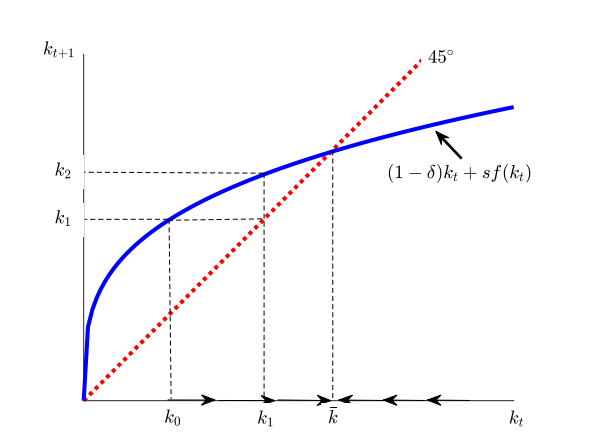
\includegraphics[width=0.8\textwidth]{figures/part1/ch1/dynamics-solow.png}
    \caption{索洛模型的动态}
    \label{dynamics-solow}
\end{figure}

直觉上讲，收敛的原因在于生产函数关于资本的边际报酬递减（\cref{as-F-quasiconcave}）。根据资本运动方程：
\begin{equation*}
    k_{t+1}-k_{t} = i_t - \delta k_t
\end{equation*}
有两种相反力量影响资本的运动：总投资和折旧。给定外生储蓄率，当资本存量较低时，单位资本的产出较高，
$i_t=sf(k_t)$相对于折旧的资本更高，从而资本存量逐渐提高。但在这一过程中，由于资本边际报酬递减，单位资本的产出逐渐降低，
当$k_t$足够大时，对应资本存量下的总投资不再能覆盖折旧，资本存量最终达到稳态。
进一步将资本运动方程变换为增长率形式：
\begin{equation*}
    \frac{k_{t+1}-k_t}{k_t} = \frac{s f\left(k_t\right)}{k_t}-\delta
\end{equation*}
根据$f^{\prime\prime}(k_t)<0$和$f(0)=0$的假设，$f(k_t)/k_t$关于$k_t$递减，这带来了投资对于资本存量的推动和
折旧随资本存量水平提高而增加这两种相反力量。


% 1.2.3 ===== Balanced Growth =====
\subsection{技术进步与平衡增长路径}

在基础模型中，我们省去了技术进步$A_t$和劳动投入$L_t$，经济在长期达到恒定稳态。在本节，我们引入两个新的特征：
一是允许劳动投入$L_t$（人口乘人均工时）随时间增长；二是引入技术进步$A_t$。从而生产函数形式为：
\begin{equation*}
    Y_t = F\left(K_t, A_tL_t\right)
\end{equation*}
也就是说，技术进步表现为劳动投入的改善。$A_tL_t$通常被称为\textbf{有效劳动}（Efficiency Labor）；
这一形式的技术进步被称为\textbf{劳动增广型}或\textbf{哈罗德中性}（Harrod-Neutral）。
\footnote{事实上，劳动增广型技术进步是唯一与平衡增长相合的技术进步形式（即所有总量变量以相同速率增长）。}
假设技术$A_t$的进步率为$\gamma$，劳动投入$L_t$的增长率为$n$。
\footnote{$n$可能有两个来源：一是人口的变化；二是人均工时的变化。}
总量形式的资本运动方程为：
\begin{equation*}
    K_{t+1}=(1-\delta) K_t+s F\left(K_t, A_t L_t\right)
\end{equation*}
由于技术进步的存在，显然是不存在上面所看到的严格意义的稳态的。
不过，通过正则化相关变量，我们能够将其转化为\textbf{平稳的变量}。两边同时除以有效劳动$A_tL_t$：
\begin{equation*}
    \frac{K_{t+1}}{A_t L_t}=(1-\delta) \frac{K_t}{A_t L_t}+s \frac{F\left(K_t, A_t L_t\right)}{A_t L_t}
\end{equation*}
通常称这一正则化后的变量为有效人均劳动，记为：
\begin{equation*}
    \tilde{k}_t \equiv \frac{K_t}{A_tL_t}
\end{equation*}
从而资本运动方程可以改写为\textbf{有效人均形式}：
\begin{equation*}
    \frac{A_{t+1}}{A_t} \frac{L_{t+1}}{L_t} \frac{K_{t+1}}{A_{t+1} L_{t+1}}=(1-\delta) 
        \frac{K_t}{A_t L_t}+s F\left(\frac{K_t}{A_t L_t}, 1\right)
\end{equation*}
即：
\begin{equation}    \label{eq-k-law-of-motion-bgp}
    (1+\gamma)(1+n) \tilde{k}_{t+1}=(1-\delta) \tilde{k}_t+s f(\tilde{k}_t)
\end{equation}
其中，$f(\tilde{k}_t) \equiv F(\tilde{k}_t,1)$。
对正则化后的资本和上述运动方程，可以得到稳定的稳态值，进而可以再将其转化为宏观变量。

事实上，对应于基准模型下的稳态，我们使用\textbf{平衡增长路径}（Balanced Growth Path）来刻画这类带有增长特征模型的长期行为。
\footnote{部分学者仍使用稳态来表示平衡增长路径，因为正则化后的变量具有严格稳定的稳态值。}
在平衡增长路径下，$\tilde{k}_t$是常数，宏观变量如$Y_t,~K_t,~C_t$\textbf{以相同的常速率增长}。
将平衡增长路径下的有效人均资本记为：$\tilde{k}_{t+1}=\tilde{k}_t=\bar{\tilde{k}}$，它是如下方程的解：
\begin{equation*}
    (1+\gamma)(1+n) \overline{\tilde{k}}=(1-\delta) \overline{\tilde{k}}+s f(\overline{\tilde{k}})
\end{equation*}
对于转换后的平稳变量，其动态特征与基准模型相近：从任意$\tilde{k}_0$开始，$\{\tilde{k}_{t+1}\}_{t=0}^{\infty}$
单调收敛到$\bar{\tilde{k}}$。

进一步分析哈罗德中性模型中经济变量的特征。假设所有劳动力都工作1单位，即$L_t$只表示总人口，
人均产出定义为$y_t\equiv Y_t/L_t$。由于在长期$Y_t /\left(A_t L_t\right)=f(\tilde{k}_t)$
收敛到$f(\bar{\tilde{k}})$，因此人均资本收敛到：
\begin{equation*}
    y_t = f(\bar{\tilde{k}})A_t
\end{equation*}
在长期，人均产出的增长率为：
\begin{equation*}
    \frac{y_{t+1}-y_t}{y_t}=\frac{f(\bar{\tilde{k}}) A_{t+1}-f(\bar{\tilde{k}}) A_t}{f(\bar{\tilde{k}}) A_t}
        =\frac{A_{t+1}-A_t}{A_t}=\gamma
\end{equation*}
也就是说，在平衡增长路径上，人均产出以$\gamma$的速率增长，其余参数如储蓄率$s$不会影响\textbf{长期速率}。

需要注意的是，上述结果说外生储蓄率对经济没有影响：它会影响人均产出的\textbf{水平值}。
同时，当经济尚未收敛到平衡增长路径上时，外生储蓄率的水平也会影响经济短期的增长率，因为短期内$\tilde{k}_t$的变动会产生影响：
\begin{equation*}
    \frac{y_{t+1}-y_t}{y_t} = 
        \frac{f(\tilde{k}_{t+1}) A_{t+1}-f(\tilde{k}_t) A_t}{f(\tilde{k}_t) A_t} = 
            \frac{f(\tilde{k}_{t+1})}{f(\tilde{k}_t)}(1+\gamma)-1
\end{equation*}
根据有效人均形势下的资本运动方程\cref{eq-k-law-of-motion-bgp}：当$\tilde{k}_t<\bar{\tilde{k}}_t$，$\tilde{k}_t$随时间增长，
即$\tilde{k}_{t+1}>\tilde{k}_t$。此时$f(\tilde{k}_{t+1})/f(\tilde{k}_t)>1$，短期内人均产出增长率高于$\gamma$。
同理，当$\tilde{k}_t>\bar{\tilde{k}}_t$，短期内人均产出增长率小于$\gamma$。


% 1.2.4 ===== 特征事实 ====
\subsection{特征事实：数据与模型}

回顾索洛模型的动机之一：解释资本产出比的长期稳定性。在长期平衡增长路径下，$Y_t/(A_tL_t) = f(\tilde{k}_t)$
和$K_t/(A_tL_t)=\tilde{k}_t$都是常数，从而$K_t/Y_t=\tilde{k}_tf(\tilde{k}_t)$也是常数。
因此索洛模型可以解释稳定的资本产出比这一特征事实。同时，在平衡增长路径下，人均产出增速稳定为$\gamma$，
这也与特征事实相匹配。

另外一层特征事实是要素价格方面的：物质资本回报率几乎稳定。我们首先需要在模型中对其进行计算。
假设厂商在竞争市场上最大化其利润：
\begin{equation}
    \max _{K_t, A_t L_t} F\left(K_t, A_t L_t\right)-r_t K_t-w_t A_t L_t
\end{equation}
简单起见，假设消费者拥有资本并将其出售给厂商，即$r_t$代表资本回报率。根据一阶条件：\textbf{资本回报率等于资本的边际产出}，即：
\begin{equation*}
    r_t = F_1\left(K_t, A_tL_t\right) 
\end{equation*}
对$f(K_t/A_tL_t) \equiv F\left(K_t, A_tL_t\right)/(A_tL_t)$两侧同时对$K_t$微分
可知：$\frac{f^{\prime}(\tilde{k}_t)}{A_tL_t}=\frac{F_1\left(K_t, A_tL_t\right)}{A_tL_t}$，从而成立：
\begin{equation*}
    r_t = f^{\prime}(\tilde{k}_t)
\end{equation*}
在长期平衡增长路径下，$\tilde{k}_t$为常数，$f^{\prime}(\tilde{k}_t)$为常数，$r_t$也为常数，与特征事实相符。

此外，当时美国经济的另一特征事实在于劳动和资本份额的稳定性。在模型中，资本份额可以表示为$r_tK_t/Y_t$，
由于我们已经证明了$K_t/Y_t$和$r_t$在长期平衡增长路径下都是稳定的，因此模型中资本份额的长期特征也能与特征事实相匹配。
对于劳动份额，在模型中可以表示为$w_tA_tL_t/Y_t$。由厂商问题的一阶条件：
\begin{equation*}
    w_t = F_2\left(K_t, A_tL_t\right)
\end{equation*}
同时，对于规模报酬不变的生产函数，它是一次齐次的，即：
\begin{equation*}
    qF\left(K_t,A_tL_t\right) = F\left(qK_t,qA_tL_t\right)
\end{equation*}
两边同时对$q$微分：
\begin{equation*}
    F\left(K_t,A_tL_t\right) = K_tF_1\left(qK_t,qA_tL_t\right) + A_tL_tF_2\left(qK_t,qA_tL_t\right)
\end{equation*}
由于上式恒成立，因此在$q=1$处有：
\begin{equation*}
    Y_t = F\left(K_t,A_tL_t\right) = K_tF_1\left(K_t,A_tL_t\right) + A_tL_tF_2\left(K_t,A_tL_t\right)
\end{equation*}
结合劳动的一阶条件，并将两边同时除以$Y_t$，可知劳动份额等于1减去资本份额：
\begin{equation*}
    w_tA_tL_t/Y_t = 1 - r_tK_t/Y_t
\end{equation*}
实际上，与证明资本份额类似，通过直接计算的方式也可以得到模型中劳动份额的特征。
对$f(K_t/A_tL_t) \equiv F\left(K_t, A_tL_t\right)/(A_tL_t)$两侧同时对$A_tL_t$微分可知：
\begin{equation*}
    -\frac{f^{\prime}(\tilde{k}_t)K_t}{(A_tL_t)^2} 
        = \frac{F_2(K_t,A_tL_t)A_tL_t - F\left(K_t, A_tL_t\right)}{(A_tL_t)^2}
\end{equation*}
结合一阶条件可得：
\begin{equation*}
    w_t = f(\tilde{k}_t) - \tilde{k}_tf^{\prime}(\tilde{k}_t)
\end{equation*}
在平衡增长路径下$\tilde{k}_t=\bar{\tilde{k}}$，工资为常数，从而资本份额$w_tA_tL_t/Y_t=w_t/f(\tilde{k}_t)$为常数，
与特征事实相符。特别的，对柯布-道格拉斯生产函数$Y_t=K_t^{\alpha}(A_tL_t)^{1-\alpha}$，即使在平衡增长路径外，
资本和劳动份额始终恒定为$\alpha$和$1-\alpha$。


% 1.2.5 ===== 收敛性分析 ===== 
\subsection{收敛性分析}

我们已经看到，在索洛模型中，经济会单调收敛至稳态或平衡增长路径。在本小节，我们对收敛性进行一些更详细的说明。
回忆最简单的基准情形，我们将劳动投入$L_t$正则化为1，以人均形式描述经济过程。
由一阶泰勒展开，资本运动方程\cref{eq-k-law-of-motion}在\textbf{稳态附近}可以进行如下估计：
\begin{equation}
    \Delta k_{t+1}=\left(1-\delta+s f^{\prime}(\bar{k})\right) \Delta k_t
\end{equation}
其中$\Delta k_{t}$表示$k_t$对其稳态值的偏离（当偏离很小时），即$k_t-\bar{k}$。两边同除以$\bar{k}$得到：
\begin{equation}
    \frac{k_{t+1}-\bar{k}}{\bar{k}}=(1-\lambda) \frac{k_t-\bar{k}}{\bar{k}}
\end{equation}
其中，$\lambda = \delta - sf^{\prime}(\bar{k})$表示\textbf{收敛速度}。
$\lambda$越大，$\Delta k_{t+1}$缩小（绝对值）得更快，即系统向稳态收敛速度快。
如\cref{fig-convergence-speed}所给出的，$\lambda$越大，资本运动方程在稳态附近斜率更平，更快到达稳态。
假设柯布-道格拉斯生产函数，一阶展开可写为：
\begin{equation}
    \Delta k_{t+1}=\left(1-\delta(1-\alpha)\right) \Delta k_t
\end{equation}
收敛速度方程为：
\begin{equation}
    \lambda = \delta(1-\alpha)
\end{equation}
因此，资本份额$\alpha$越低、折旧率$\delta$越大，则收敛速度越快。

\begin{figure}
    \centering
    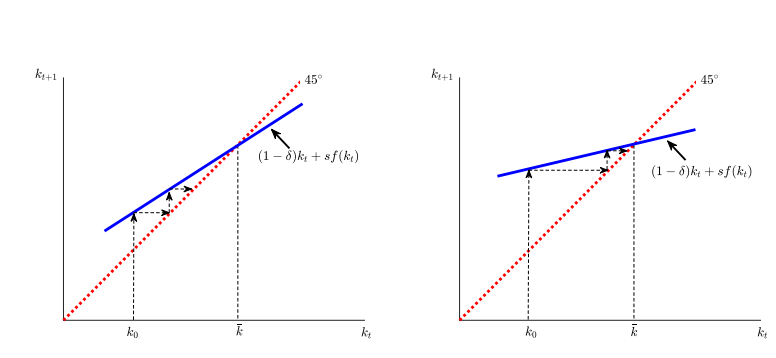
\includegraphics[width=1\textwidth]{figures/part1/ch1/convergence-speed.png}
    \caption{收敛速度}
    \label{fig-convergence-speed}
\end{figure}

一般而言，$k_t$如何影响$k_{t+1}$决定了收敛速度。例如，若$k_t$对$k_{t+1}$无影响，那么收敛会立刻实现，
即在\cref{fig-convergence-speed}反应为水平的直线。
不难看出，外生储蓄率$s$在柯布-道格拉斯生产函数下不会影响收敛速度，这是两个相反力量所导致的：
对给定的一个$k_t$，高的储蓄率$s$意味着$k_t$对$k_{t+1}$的影响更大；但更高的储蓄率也带来更高的稳态$\bar{k}$，
进而稳态时资本的边际产出$f^{\prime}(\bar{k})$低，这意味着$k_t$对$k_{t+1}$的影响更小。
在CD生产函数下，这两种作用相互抵消。

进一步回忆带有增长特征的索洛模型：
对其有效人均形式的资本运动方程\cref{eq-k-law-of-motion-bgp}在稳态附近进行一阶泰勒展开可得：
\begin{equation}
    (1+\gamma)(1+n) \Delta \tilde{k}_{t+1}
        = \left(1-\delta+s f^{\prime}(\overline{\tilde{k}})\right) \Delta \tilde{k}_t
\end{equation}
两边同时除以$\bar{\tilde{k}}$，得到收敛速度方程：
\begin{equation*}
    \frac{\tilde{k}_{t+1}-\bar{\tilde{k}}}{\tilde{\tilde{k}}}
        = (1-\lambda) \frac{\tilde{k}_t-\bar{\tilde{k}}}{\tilde{\tilde{k}}}
\end{equation*}
其中收敛速度为：
\begin{equation*}
    \lambda=1-\frac{1-\delta+s f^{\prime}(\bar{\tilde{k}})}{(1+\gamma)(1+n)} 
\end{equation*}
类似的，在柯布-道格拉斯生产函数下，一阶展开可写为：
\begin{equation*}
    \Delta \tilde{k}_{t+1}
        = \left(\alpha+\frac{(1-\alpha)(1-\delta)}{(1+\gamma)(1+n)}\right) \Delta \tilde{k}_t
\end{equation*}
收敛速度为：
\begin{equation*}
    \lambda = (1-\alpha)\left(1-\frac{1-\delta}{(1+\gamma)(1+n)}\right)
\end{equation*}


% 1.2.6 ===== 增长核算 ===== 
\subsection{应用索洛模型：增长核算}

更一般化的，Solow（1957）提出增长核算（Growth Accounting）的概念，用于研究不同生产要素对经济增长的作用。假设如下：
\begin{assumption}
    总产出$Y_t$由总量生产函数$F_t\left(K_t,L_t\right)$决定，$F$的时间记号保留了技术进步促进生产函数向上移动的可能；
\end{assumption}
\begin{assumption}
    $F$规模报酬不变及其余新古典性质；
\end{assumption}
\begin{assumption}
    投入要素完全竞争，即厂商最大化其利润。
\end{assumption}

微观经济学证明了，在完全竞争均衡情形下，规模报酬不变最终带来\textbf{零利润}，这也是索洛增长核算的起点。
与前面的记号类似，以小写字母表示人均测度，假设人口总量为$N_t$，根据规模报酬不变，我们可以将\textbf{人均产出}
表示为$y_t=F_t\left(k_t,l_t\right)$，其中$k_t\equiv K_t/N_t$和$l_t\equiv L_t/N_t$表示人均资本和人均工作时间。
假设人口总量不变，并将其正则化为1，可以得到$y_t=Y_t$。
\footnote{在基准模型中，我们额外假设了人均工时为常数，进而将其也正则化为1，因此基准模型是没有考虑劳动的。}
对此处的人均产出进行全微分可得：
\begin{equation}
    \begin{aligned}
        dy &= \frac{\partial F}{\partial t}dt + \frac{\partial F}{\partial k}dk + \frac{\partial F}{\partial l} \\
            &=  \frac{\partial F}{\partial t}dt 
                + \frac{\partial F}{\partial k} k \frac{dk}{k} + \frac{\partial F}{\partial l} l \frac{dl}{l}
    \end{aligned}
\end{equation}
其中所有的全微分都在$\left(t,k_t,l_t\right)$处取得。
在此处，为了方便取导数，我们假设了时间连续，但离散情形下并没有本质区别，只是记号的差异。
记$r_t, w_t$为完全竞争市场上的资本租金率和工资，厂商最大化利润问题为：
\begin{equation*}
    \max _{k, \ell} F_t(k, \ell)-r k-w l
\end{equation*}
根据一阶条件可得：
\begin{align}
    r &= \partial F / \partial k \\
    w &= \partial F / \partial l
\end{align}
两边同时除以总产出可得：
\begin{equation}
    \frac{d y}{y} = \frac{\partial F}{\partial t} 
        \frac{d t}{y} + \frac{r k}{y} \frac{d k}{k} + \frac{w l}{y} \frac{d l}{l}
\end{equation}
假设$1-\alpha$为劳动收入份额（可能时变，根据数据可计算），那么由规模报酬不变的零利润条件可知：资本份额为$\alpha$，
从而得得如下\textbf{增长核算方程}：
\begin{equation}
    \frac{d y}{y}=\frac{\partial F}{\partial t} \frac{d t}{F}+\alpha \frac{d k}{k}+(1-\alpha) \frac{d l}{l}
\end{equation}
其中，$\frac{\partial F}{\partial t}\frac{dt}{F}$被称为\textbf{索洛剩余}（Solow Residual），
因为它是不能由资本和劳动增长核算得到的部分，但可以通过作差得到，它测度了生产可能前沿如何随时间变动。

上述形式是一般化地将时间对生产函数的影响进行表示。我们可能对以下形式更为熟悉：
$F_t\left(k_t, l_t\right) \equiv A_tF\left(k_t, l_t\right)$，
由于$F$为一次齐次，因此这一形式被称为\textbf{希克斯中性}（Hicks-Neutral），
$A$被称为\textbf{全要素生产率}（Total Factor Productivity，TFP）。
$F\left(k_t,l_t\right)$是时间独立的函数，通过全微分可得到核算方程为：
\begin{equation}
    \frac{d y}{y}=\frac{d A}{A}+\alpha \frac{d k}{k}+(1-\alpha) \frac{d l}{l}
\end{equation}
若生产函数形式是\textbf{哈罗德中性}：$F_t\left(k_t, l_t\right) = F\left(k_t, A_tl_t\right)$，
此时$F$也是时间独立的，由厂商一阶条件$\frac{\partial F}{\partial l}=w/A$以及$wl=(1-\alpha)F$，
可类似的得到增长核算方程：
\begin{equation}
    \frac{d y}{y}=(1-\alpha) \frac{d A}{A}+\alpha \frac{d k}{k}+(1-\alpha) \frac{d l}{l}
\end{equation}

% 1.3 =============== 最优增长模型 ===============

\section{最优增长：RCK模型} \label{sec-opt-growth}

Solow（1956）和Swan（1956）的工作标志新古典增长理论的诞生。但Solow模型的主要问题在于，模型中储蓄率是外生给定的。
Cass（1965）和Koopmans（1965）在Solow工作的基础上，通过引入微观基础对新古典理论进行了拓展，
建立了确定性情形下的\textbf{最优增长模型}：他们利用家庭偏好来解释为何储蓄是一种内生理性选择的结果。
最优增长模型通常被称为RCK模型（Ramsey-Cass-Koopmans Model），它与消费-储蓄模型的核心区别在于：经济是生产经济而不是禀赋经济。
我们将利用这一模型，深入研究序列视角下的动态优化问题。

典型的确定性最优增长模型形式如下：假设时间是离散且无穷的，由$t=0,1,\dots, \infty$表示，第0期资本存量$k_0>0$给定。
生产函数$F$与索洛模型中类似，具有新古典特征，同样假设总劳动投入被正则化为$L=1$，从而人均形式生产函数为：$y_t=f(k_t)$。
不难证明，索洛模型对$F$的假设对$f$同样成立：
\begin{assumption} \label{as-f}
    $f$关于$k$严格增
\end{assumption}
\begin{assumption}
    $f$关于$k$严格拟凹
\end{assumption}
\begin{assumption}
    f(0)=0
\end{assumption}
\begin{assumption} \label{as-f-inada}
    生产函数Inada条件：
        $\lim\limits_{k \rightarrow 0} f^{\prime}(k)=\infty, \quad \lim\limits_{k \rightarrow \infty} f^{\prime}(k)=0$
\end{assumption}
\begin{assumption}
    方便起见额外假设：$f\left(k\right)$连续，二次可微。
\end{assumption}
计划者（Social Planner）（或代表性家庭）在资源约束:
$$c_t+k_{t+1}=f\left(k_t\right)+(1-\delta)k_t,\quad \forall t \geq 0$$
和资源非负的约束下：
$$c_t \geq 0, \quad k_{t+1} \geq 0, \quad \forall t \geq 0$$
选择无穷期序列：
$$\left\{c_t, k_{t+1}\right\}_{t=0}^{\infty}$$
来最大化效用函数：
$$\sum_{t=0}^{T} \beta^t u\left(c_t\right)$$
其中$T$可以取无穷。这一形式的问题通常被称为\textbf{序列问题（Sequence Probem）}。
同时，模型对效用函数也有类似生产函数的的规范化假设：
\begin{assumption} \label{as-u}
    效用函数$u$连续，二次可微
        且$u^{\prime}\left(c\right)>0,\quad u^{\prime\prime}\left(c\right)<0$
\end{assumption}
\begin{assumption} \label{as-u-inada}
    效用函数Inada条件：
    $\lim\limits_{c \rightarrow 0} u^{\prime}(c)=\infty, \quad \lim\limits_{c \rightarrow \infty} U^{\prime}(c)=0$
\end{assumption}

利用Lagrangian函数是处理类似优化问题的基本方法。但当问题拓展到上面无穷期形式时，需要一些额外条件来确保问题的可解性。
我们将从有限期情形开始，逐步推广至无限期的情形。


% 1.3.1 ===== 有限期情形 =====
\subsection{有限期情形} \label{subsec-finite-h}

首先考虑上面问题的有限期形式，
即时间$t \in$ $\{0,1, \ldots T\}$。对于最大化问题，记第$t$期资源约束相关的乘子为$\beta^t \lambda_t$，进而可构造如下拉格朗日方程：
$$
\mathcal{L}=\sum_{t=0}^T \beta^t u\left(c_t\right)-\sum_{t=0}^T \beta^t \lambda_t\left[c_t+k_{t+1}-(1-\delta) k_t-f\left(k_t\right)\right]
$$
也即：
$$
\mathcal{L}=\sum_{t=0}^T \beta^t\left\{u\left(c_t\right)-\lambda_t\left[c_t+k_{t+1}-(1-\delta) k_t-f\left(k_t\right)\right]\right\}
$$
不难看出，$\lambda_t$是计划者第$t$期资源约束的影子价格，或者说是边际价值。在生产函数和效用函数满足规范化假设时，只要$k_t>0$，这一问题有内点解。
分别对$c_t$和$k_{t+1}$求一阶条件，可得：
$$u^{\prime}\left(c_t\right)-\lambda_t=0$$
$$-\lambda_t+\beta\lambda_{t+1}\left[1-\delta+f^{\prime}\left(k_{t+1}\right)\right]=0$$
与乘子$\lambda_t$相关的一阶条件即为资源约束：在第$t$期，如果经济额外获得$\epsilon$足够小单位的商品，那么从第$t$期看，
福利增加了$\lambda_t\epsilon$；从第0期看，则福利增加了$\beta^t\lambda_t$单位。
合并两个一阶条件可得：
$$
\frac{u^{\prime}\left(c_t\right)}{\beta u^{\prime}\left(c_{t+1}\right)}=f^{\prime}\left(k_{t+1}\right)+1-\delta
$$
这一条件表明：计划者的最优选择是使得今明两天消费的MRS与MRT相等

对于资本$k$，一个自然的问题是：
终期$T$时如何选择，即$k_{T+1}$的最优值?由$k_{T+1}$的KT条件:
$$\frac{\partial \mathcal{L}}{\partial k_{T+1}} \geq 0, \quad k_{T+1} \geq 0$$
且满足互补松弛条件。这等价于：
$$
\beta^T \lambda_T \geq 0, \quad k_{T+1} \geq 0, \quad \beta^T \lambda_T k_{T+1}=0
$$
这意味着在终期第$T$期选择的$k_{T+1}=0$或$k_{T+1}$的影子价值为0，因为不存在$T+1$期，从而在第$T$期选择$k_{T+1}$没有意义。
又由于$\lambda_T=u^{\prime}\left(c_T\right)$，而模型\textbf{假设}$u^{\prime} > 0$，因此，终期T存在角点解：
$$k_{T+1}=0$$
或者说，如果终期选择$k_{T+1}>0$，则计划者会余下未使用资源，在规范化假设下这不会是最优策略（因为$u^{\prime}>0$）。


% 1.3.2 ===== 无限期情形 =====
\subsection{无限期情形} \label{subsec-infinit-h}

现在，\textbf{由有限期转向无限期问题}。回忆在有限期问题中，终期时$k_{T+1}$的最优条件满足：
$$\beta^T \lambda_T k_{T+1}=0$$
从直觉出发，令$T \rightarrow \infty$，那么可以得到无限期情形下的\textbf{横截性条件}（Transversality Condition）：
\begin{equation}
    \lim _{T \rightarrow \infty} \beta^T \lambda_T k_{T+1}=0
\end{equation}
\textbf{这一条件排除了无限期情形下资本无限增长的可能性}。计划者的最优配置$\left\{c_t, k_{t+1}\right\}_{t=0}^{\infty}$是符合
如下欧拉方程（optimality）、资源约束（feasibility）和边界条件的一条\textbf{唯一路径}（unique path）：
\begin{equation}    \label{eq-euler-sp}
    \frac{u^{\prime}\left(c_t\right)}{\beta u^{\prime}\left(c_{t+1}\right)}=f^{\prime}\left(k_{t+1}\right)+1-\delta
\end{equation}
\begin{equation}    \label{eq-res-const-sp}
    k_{t+1}=f\left(k_t\right)+(1-\delta) k_t-c_t
\end{equation}
以及两个边界条件
$$
k_0>0, \quad \lim _{t \rightarrow \infty} \beta^t u^{\prime}\left(c_t\right) k_{t+1}=0
$$
式\eqref{eq-euler-sp}被称为\textbf{欧拉方程（Euler Equation）}。
事实上，符合前两条条件的$\left\{c_t, k_{t+1}\right\}_{t=0}^{\infty}$路径可能有多条，但在两个边界条件约束下，这条路径是唯一确定的。后续将会证明。
% 第2章 动态宏观经济学的基本方法与概念

% 导言

\chapter{递归方法与动态规划} \label{ch-dynamic-opt-fe-dp}

第一章提出了处理动态优化问题的两个视角：序列视角和递归视角，并对序列化求解进行了介绍。
本章从递归的视角对动态优化问题进行进一步研究。
我们继续借助最优增长模型：将原始的序列问题转化为递归形式，建立贝尔曼方程，引入确定性动态规划的基本理论方法；
接着，对序列问题和递归形式的关系进行研究，证明解的存在性和其他相关相应性质；
最后介绍模型的线性解法并初步讲解数值解法，为后续学习奠定基础。


% =============== main ch2 ===============


% 2.1 ===== 递归与动态规划基本概念 =====
% 2.1 =============== 递归与动态规划的基本概念 ===============

\section{递归与动态规划的基本概念}  \label{sec-fe-dp-concept}

对于第一章中所要求解的动态优化问题，我们的目标是寻找一个最优值序列，通常我们把这样的问题称为\textbf{序列问题}。
但这一问题形式的求解存在一定不足：处理无限期情形过于复杂，将面临无穷的差分方程序列，我们希望降维。
Stocky、Lucas等人基于贝尔曼建立的动态规划理论，将序列问题转化为递归形式求解，由此建立了现代宏观的核心方法，
而递归也成为绝大多数宏观模型的核心特征。

具体看：无穷序列问题可以分解为一期一期的小问题：对于$t+1$期，可以在第$t$期进行选择而不用在第0期进行，即定义从当期到下期的映射，
这一问题形式被称为\textbf{递归形式}（Recursive Formulation）。
\textbf{序列问题求解后，我们得到了无穷个数值（Number）；对于递归问题，我们求解所得的是一个方程（Function）,其本质是一个泛函问题}。
利用泛函方程（Function Equation）对动态优化问题进行研究就是\textbf{动态规划}（Dynamic Programmming），
这一概念最早由Richard E. Bellman提出。在本节，我们将建立一般化形式的递归问题，进而对动态规划中的基本概念进行初步介绍。


% 2.1.1 ===== sq-fe =====
\subsection{由序列问题转向递归形式}

回忆第\ref{ch-dynamic-opt-sq}章建立的一般化形式的动态优化问题\cref{problem-general-dynamic-opt}：
\begin{equation*}
    \begin{aligned}
        \max _{\left\{y_t, x_{t+1}\right\}_{t=0}^T} & \sum_{t=0}^T \beta^t \hat{\mathcal{F}}\left(y_t\right) \\
        \text { s.t. } & x_{t+1}=h\left(x_t, y_t\right) \\
        & x_{t+1} \in \Gamma\left(x_t\right) .
    \end{aligned}
\end{equation*}
利用$x_{t+1}=h(x_t,y_t)$，可将控制变量$y_t$表示为$y_t = \hat{h}(x_t,x_{t+1})$，将其替换到目标函数中，记
$\mathcal{F}(x_t,x_{t+1})\equiv \hat{\mathcal{F}}\left(\hat{h}(x_t,x_{t+1})\right)$，从而无穷期序列问题可写为：
\begin{equation*}
    \max _{\left\{x_{t+1} \in \Gamma\left(x_t\right)\right\}_{t=0}^{\infty}}
        \sum_{t=0}^{\infty} \beta^t \mathcal{F}\left(x_t, x_{t+1}\right)
\end{equation*}
在序列问题形式下，我们在初始时刻选择$x_{t+1}$的全部路径；
而递归问题和动态规划的核心想法是：\textbf{动态决策不是一次全部做出的，而是一期一期进行的}，
即$x_{t+1}$的值不是在第0期而是在第$t$期决定的。为了使这一想法更清晰，我们将最优化的序列问题记为：
\begin{equation}    \label{eq-def-value-func}
    v\left(x_0\right) \equiv 
        \max _{\left\{x_{t+1} \in \Gamma\left(x_t\right)\right\}_{t=0}^{\infty}} 
        \sum_{t=0}^{\infty} \beta^t \mathcal{F}\left(x_t, x_{t+1}\right)
\end{equation}
给定$x_t$，$\Gamma(x_t)$是$x_{t+1}$的可行集。
在这一表达式中，我们称$V(x_0)$为\textbf{值函数}（Value Function），它代表给定起初条件$x_0$，取最优处时目标函数的值。
我们可以将这一高维问题化简降维：
\begin{equation}
    \begin{aligned}
        v\left(x_0\right) &= \max _{\left\{x_{t+1} \in \Gamma\left(x_t\right)\right\}_{t=0}^{\infty}}
            \left\{\mathcal{F}\left(x_0, x_1\right) + 
                \beta \sum_{t=1}^{\infty} \beta^{t-1} \mathcal{F}\left(x_t, x_{t+1}\right)\right\} \\
        &= \max _{x_1 \in \Gamma\left(x_0\right)}
            \left\{\mathcal{F}\left(x_0, x_1\right) + 
                \beta\left[\max _{\left\{x_{t+1} \in \Gamma\left(x_t\right)\right\}_{t=1}^{\infty}} 
                    \sum_{t=1}^{\infty} \beta^{t-1} \mathcal{F}\left(x_t, x_{t+1}\right)\right]\right\} \\
        &= \max _{x_1 \in \Gamma\left(x_0\right)}
            \{\mathcal{F}\left(x_0, x_1\right) + 
                \beta \underbrace{\left[\max _{\left\{x_{t+2} \in \Gamma\left(x_{t+1}\right)\right\}_{t=0}^{\infty}}
                    \sum_{t=0}^{\infty}\beta^t\mathcal{F}\left(x_{t+1},x_{t+2}\right)\right]}_{\equiv v\left(x_1\right)}\}
    \end{aligned}
\end{equation}
其中利用了$\max_{x,y}f(x,y) = \max_{y}\{\max_{x}f(x,y)\}$。
注意到，最后一行等式的中括号中最大化问题的结构和\cref{eq-def-value-func}完全相同，唯一不同的是初始条件变为了$x_1$。
换句话说，它代表给定初始条件为$x_1$时，决策者选择最优序列$x_{t+1}$下目标函数的值。
由于时间是无穷的，并且当期目标函数和可行集$\Gamma$都不随时间改变，因此中括号中的表达式正是$V(x_1)$，进而我们得到：
\begin{equation*}
    v\left(x_0\right) = 
        \max _{\left\{x_1 \in \Gamma\left(x_0\right)\right\}}\left\{\mathcal{F}\left(x_0, x_1\right) + 
            \beta v\left(x_1\right)\right\}
\end{equation*}

一个自然的问题是：序列问题和递归问题的两种表达形式等价吗？答案是，只要问题是\textbf{平稳的}（Stationary），等价性就存在。
直观上讲，但只要第$t$期的问题和$t+1$期的问题结构相同，动态优化问题就是平稳的，
或者说，决策者所有决策相关的信息都与时间无关。因此，平稳性实际包括另一层含义：\textbf{值函数不依赖于时间}。
实际上，并非所有问题都是平稳的，例如在有限期的最优增长模型中，计划者选择资本时会关注剩余的时间。随着终期接近，决策问题也随之变化。
此时，问题虽然仍可表征为递归形式，但值函数会依赖于时间，即$v_t$。而在无限期情形下，任意时刻后剩余的时间都是相同的。
虽然决策会随值函数自变量的不同而改变，但不会受作出这一决策的时刻的影响，在任意时刻与决策唯一相关的就是当期的资本水平。


% 2.1.2 ===== 贝尔曼方程 =====
\subsection{状态变量、贝尔曼方程与决策规则}

一般，我们称对决策者而言前定的（Predetermined）、回报相关度（Payoff-Relevant）的信息为\textbf{状态变量}（State Variable）。
例如最优增长模型中的当期资本存量$k_t$、一般化形式问题中的$x_t$。当我们把序列问题转化为递归问题时，
选择合适的状态变量来确保转化后的问题确实具有递归形式是十分重要的。当问题是平稳的，决策的形式也是平稳的：
\begin{equation*}
    x_{t+1} = g(x_t)
\end{equation*}
即决定未来资本如何依赖于档期状态的函数不依赖于时间。我们称函数$g(\cdot)$为\textbf{决策规则（}Decision Rule）或
\textbf{策略函数}（Policy Function）。

对任意给定的初始条件$x_t$，我们可以将递归问题写为：
\begin{equation*}
    v\left(x_t\right) = 
        \max _{x_{t+1} \in \Gamma\left(x_t\right)}
        \left\{\mathcal{F}\left(x_t, x_{t+1}\right)+\beta v\left(x_{t+1}\right)\right\}
\end{equation*}
这一问题形式被称为\textbf{动态规划}（Dynamic Programming）。
不难看出，对平稳的无限期问题是，那么时间记号并不重要，以记号$x$表示状态变量的当期值，以记号$x^{\prime}$表示下期值，
从而动态规划问题为：
\footnote{我们也可以将贝尔曼方程形式写为如下形式$v(x)=\max _{y \in \Gamma(x)}\left\{\mathcal{F}\left(x, y\right)
+\beta v\left(x^{\prime}\right)\right\}$，只是记号差异，分析并没有本质不同。
因为一旦确定了$y_t$，就相当于确定了$x_{t+1}$。我们在后面将频繁看到这一记号的使用。}
\begin{equation}    \label{eq-dp-bellman}
    v(x) = \max _{x^{\prime} \in \Gamma(x)}
        \left\{\mathcal{F}\left(x, x^{\prime}\right)+\beta v\left(x^{\prime}\right)\right\}
\end{equation}
这一方程就是\textbf{贝尔曼方程}（Bellman Equation）。
注意到，方程左右两侧都包含值函数$V(\cdot)$，但是我们并不知道其具体形式，即方程的未知量是函数$v(\cdot)$:
对任意$x$，$v(\cdot)$都需满足\cref{eq-dp-bellman}。因此，贝尔曼方程本质是一个\textbf{泛函方程}（Functional Equation）。
记函数$g(\cdot)$使贝尔曼方程取最大化，即：
\begin{equation*}
    g(x) = \arg \max _{x^{\prime} \in \Gamma(x)}
        \left\{\mathcal{F}\left(x, x^{\prime}\right)+\beta v\left(x^{\prime}\right)\right\}
\end{equation*}
因此对所有$x$，下期$x^{\prime}$的决策规则为：$x^{\prime}=g(x)$。
需要注意，在当前记号下，我们实际假定了最大值存在并且唯一。否则，$g$可能不存在或者说不是一个函数而是对应（Corresponsence）。


% 2.1.3 ===== 欧拉泛函 =====
\subsection{欧拉泛函}

在序列问题下，通过求解一阶条件得到的欧拉方程是刻画解特征的关键。
自然的，我们希望通过对贝尔曼方程求解一阶条件来寻找决策规则的特征。但是一个核心问题在于:
我们并不知道$v$的形式，进而也不知道$v^{\prime}$的形式，求解得到一阶条件难以发挥作用。具体看，对如下贝尔曼方程：
\begin{equation*}
    v(x)=\max _{x^{\prime} \in \Gamma(x)}
        \left\{\mathcal{F}\left(x, x^{\prime}\right)+\beta v\left(x^{\prime}\right)\right\}
\end{equation*}
若\textbf{假设值函数$v\left(\cdot\right)$已知}，那么贝尔曼方程就被就简化为一个两期优化问题：
\begin{equation*}
    \max _{x^{\prime} \in \Gamma(x)}
        \left\{\mathcal{F}\left(x, x^{\prime}\right)+\beta v\left(x^{\prime}\right)\right\}
\end{equation*}
对$x^{\prime}$求导可得\textbf{一阶条件}：
\begin{equation}   \label{eq-bellman-foc} 
    \mathcal{F}_2(x,x^{\prime}) + \beta v^{\prime}(x^{\prime}) = 0
\end{equation}
也就是说，内点解必须满足上式。假设存在决策规则$g(x)$是内点解，因此有：
\begin{equation}   \label{eq-bellman-foc-opt}
    \mathcal{F}_2\left(x, g(x)\right) + \beta v^{\prime}\left(g(x)\right)=0
\end{equation}
但是，在对$v$或$v^{\prime}$有更多了解前，我们无法做更多分析。幸运的是，利用\textbf{包络定理}可以解决这一问题。

注意到，根据决策规则的定义，在最优处时（$x^{\prime} = g(x)$）最大化算子消失，下式对所有$x$恒成立：
\begin{equation}    \label{eq-bellman-opt}
    v(x)=\mathcal{F}(x, g(x))+\beta v(g(x))
\end{equation}
对其两侧同时关于$x$全微分得到：
\begin{equation*}
    v^{\prime}(x) = \mathcal{F}_1(x, g(x))
        +\underbrace{g^{\prime}(x)\left[\mathcal{F}_2(x, g(x))
        +\beta v^{\prime}(g(x))\right]}_{\text {间接效应 } }
\end{equation*}
策略函数导数的出现似乎使问题变得更加复杂，但根据一阶条件的最优性（即\cref{eq-bellman-foc-opt}），中括号中的项正为0，
从而我们得到：
\begin{equation*}
    v^{\prime}(x) = \mathcal{F}_1\left(x,g(x)\right)
\end{equation*}
实际上，$x$的变动对值函数有两方面影响：一方面是直接对当期目标函数产生作用；
另一方面是其导致决策规则变化，进而间接影响未来的效用，然而一阶条件的最优性使得间接效用消失——这本质上是\textbf{包络定理}的运用。
在动态规划问题中，上述条件也被称为\textbf{Benveniste-Schenkman条件}。

现在，我们得到了值函数导数的表达式，进而也可知
$v^{\prime}\left(g(x)\right)=\mathcal{F}_{1}\left(g\left(x\right),g\left(g\left(x\right)\right)\right)$。
因此，最优处时的一阶条件\cref{eq-bellman-foc-opt}可以进一步写为：
\begin{equation}    \label{eq-bellman-euler-fe}
    \mathcal{F}_2(x, g(x))+\beta \mathcal{F}_1(g(x), g(g(x)))=0, ~ \forall x 
\end{equation}
回顾序列问题中欧拉方程的形式：
\begin{equation*}
    \mathcal{F}_2\left(x_t, x_{t+1}\right)+\beta \mathcal{F}_1\left(x_{t+1}, x_{t+2}\right)=0, ~ \forall t
\end{equation*}
其未知成分是数值构成的序列$\{x_t\}_{t=1}^{\infty}$。
在递归形式下，\cref{eq-bellman-euler-fe}并不包含特定的未知量如$x_t,~x_{t+1},~x_{t+2}$，而是对对所有$x$成立，
\textbf{其未知是策略函数}$g$。因此，它实际是将欧拉方程表达为泛函，通常称之为\textbf{欧拉泛函}（Functional Euler Equation）。


% ===== 解法启示 =====
\subsection{对递归问题解法的启示：贝尔曼方程 vs 欧拉泛函}

对于动态优化问题,
在前一章的\textbf{序列视角下}：我们通过利用非线性差分方程（欧拉方程）和横截性条件来求解最有序列；
在本章的\textbf{递归视角下}：我们首先建立了关于值函数的贝尔曼方程：
\begin{equation*}
    v(x) = \max _{x^{\prime} \in \Gamma(x)}
        \left\{\mathcal{F}\left(x, x^{\prime}\right)+\beta v\left(x^{\prime}\right)\right\}
\end{equation*}
接着推导出了关于决策规则的欧拉泛函：
\begin{equation*}
    \mathcal{F}_2(x, g(x))+\beta \mathcal{F}_1(g(x), g(g(x)))=0, ~ \forall x
\end{equation*}
他们都是泛函方程，但前者的未知量是值函数，后者的未知量是策略函数（决策规则）。
这实际上对应了两种动态规划问题求解思路：直接利用贝尔曼方程求解值函数或利用欧拉泛函求解策略函数，
二者是不同的。通过求解值函数，我们可以进一步得到决策规则$k^{\prime} = g(k)$，这是一维动力系统；
而直接处理泛函的话，我们面对的是一个二维动力系统。在后面我们将看到，贝尔曼方程符合压缩映射定理的条件，可以迭代求得唯一解，较为稳健；
欧拉泛函并不是压缩映射，它只是最优策略函数$g$的一个必要条件，因此存在多重解的可能，但求解速度更快。

从下一节开始，我们将运用本节所介绍的思路及工具，对递归形式的RCK模型展开分析。
并且，我们将在RCK模型的基础上，深入讨论值函数性质、动态规划求解等关键问题。


% 2.2 ===== 递归形式下的RCK =====
% 2.2 =============== 递归形式下的最优增长模型 ===============

\section{递归形式下的最优增长模型}  \label{sec-rck-fe}

通常，将序列问题转化为递归形式能够帮助我们更好地进行分析。当一个动态问题被写为递归形式后，经济的行为唯一依赖的就是\textbf{状态变量}。
此外，目前已经发展出了许多与递归问题相关的方便的计算方法，我们将在后面的章节详细学习。
在本节，我们将会把无限期最优增长模型写为递归形式，基于上一节的思路和工具，深入研究动态规划的相关理论方法。


% 2.2.1 ===== 贝尔曼方程与一阶条件 =====
\subsection{贝尔曼方程与一阶条件} \label{subsec-rck-bellman-foc}

对于无限期最优增长模型，不难看出问题是平稳的，状态变量是每期的期初资本存量$k$，值函数仅依赖于$k$，
给定不同的资本存量将会得到不同的最优化序列和最优值。因此我们可以将值函数记为$v(k)$。控制变量是$c = f(k)+(1-\delta)k-k^{\prime}$。
为了记号方便，记$\gamma(k)\equiv f\left(k\right)+\left(1-\delta\right)k$，从而RCK模型的贝尔曼方程为：
\begin{equation}    \label{eq-rck-bellman}
    v\left(k\right) = \max _{k^{\prime}\in \Gamma(k)}
        \left[u\left(\gamma\left(k\right)-k^{\prime}\right)+\beta v\left(k^{\prime}\right)\right]
\end{equation}
其中，可行集$\Gamma(k) = \left[0,\gamma(k)\right],~\forall k$。记其决策规则为$k^{\prime}=g(k)$：
\begin{equation*}
    g\left(k\right) \equiv \underset{k^{\prime}\in\Gamma(k)}{\operatorname{argmax}}
        [u(\gamma\left(k\right)-k^{\prime})+\beta v\left(k^{\prime}\right)]
\end{equation*}
与上一节类似，\textbf{假设值函数$v\left(\cdot\right)$已知}，那么贝尔曼方程就被就简化为一个两期优化问题：
\begin{equation*}
    \max _{k^{\prime}\in\Gamma(k)}
        \left[u\left(\gamma\left(k\right)-k^{\prime}\right)+\beta v\left(k^{\prime}\right)\right]
\end{equation*}
对$k^{\prime}$求导可得\textbf{一阶条件}：
\begin{equation}    \label{eq-rck-bellman-foc}
    u^{\prime}\left(\gamma\left(k\right)-k^{\prime}\right) = \beta v^{\prime}\left(k^{\prime}\right)
\end{equation}
假设存在决策规则时内点解，从而$k^{\prime}=g(k)$满足一阶条件，即最优处的一阶条件为：
\begin{equation}    \label{eq-rck-bellman-foc-opt}
    u^{\prime}\left(\gamma(k)-g(k)\right) = \beta v^{\prime}\left(g(k)\right)
\end{equation}

在序列问题下，结合一阶条件和边界条件，理论上可以解得最优序列。
但是，对于递归问题，正如上一节指出的，\textbf{核心问题在于}：$v$未知，进而$v^{\prime}$也未知。换句话说，我们需要得到$v^{\prime}$。
不过我们已经知道，通过包络定理，我们可以很方便的得到$v^{\prime}$，进而得到欧拉泛函。下面进一步求解这一最优条件。


% 2.2.2 ===== Euler =====
\subsection{包络定理与欧拉泛函} \label{subsec-rck-euler-fe}

注意到，在问题取到最优，即$k^{\prime}=g\left(k\right)$时，贝尔曼方程的最大化算子消去，对任意$k$下式恒成立：
\begin{equation*}
    v\left(k\right) = 
        u\left(\gamma\left(k\right)-g\left(k\right)\right)+\beta v\left(g\left(k\right)\right),\quad \forall k
\end{equation*}
方程两边同时对$k$做微分可得：
\begin{equation}
    \begin{aligned}
    v^{\prime}\left(k\right) 
    &= u^{\prime}\left(\gamma\left(k\right)-g\left(k\right)\right)
            \left(\gamma^{\prime}\left(k\right)-g^{\prime}\left(k\right)\right)
            + \beta v^{\prime}\left(g\left(k\right)\right)g^{\prime}\left(k\right) \\
    &= u^{\prime}\left(\gamma\left(k\right)-g\left(k\right)\right)\gamma^{\prime}\left(k\right) 
            -u^{\prime}\left(\gamma\left(k\right)-g\left(k\right)\right)g^{\prime}\left(k\right) 
            + \beta v^{\prime}\left(g\left(k\right)\right)g^{\prime}\left(k\right) \\
    & = u^{\prime}\left(\gamma\left(k\right)-g\left(k\right)\right)\gamma^{\prime}\left(k\right)
            +g^{\prime}\left(k\right)\left[-u^{\prime}\left(\gamma\left(k\right)-g\left(k\right)\right)
            +\beta v^{\prime}\left(g\left(k\right)\right)\right] \\
    &= \underbrace{u^{\prime}\left(c\right)\left[f^{\prime}\left(k\right)
            +\left(1-\delta\right)\right]}_{\text{k变化的直接效应}}
            + \underbrace{\left[-u^{\prime}\left(c\right)+\beta v^{\prime}\left(g\left(k\right)\right)\right]
            g^{\prime}\left(k\right)}_{\text{选择最优$k^{\prime}=g\left(k\right)$的间接效应}}
    \end{aligned}
\end{equation}
由于决策规则满足一阶条件，即有\cref{eq-rck-bellman-foc-opt}成立
将其带入全微分的恒等式,发现右侧第二项中括号部分为0——即由选择最优$k^{\prime}=g(k)$带来的间接影响为0，进而得到值函数导数为：
\begin{equation}    \label{eq-rck-v-prime}
    \begin{aligned}
        v^{\prime}\left(k\right) &= 
            u^{\prime}\left(\gamma\left(k\right)-g\left(k\right)\right)\gamma^{\prime}\left(k\right) \\
        &\equiv u^{\prime}\left(c\right)\left[f^{\prime}\left(k\right)+1-\delta\right] 
    \end{aligned}
\end{equation}
同样，推导过程实际就是\textbf{包络定理}的应用：状态变量$k$的变化会通过两条途径影响值函数：
\begin{itemize}
    \item 直接路径：$k$变化-当期产出$f\left(k\right)$变化-消费$c$变化
    \item 间接路径：$k$变化-最优选择$k^{\prime}$变化-影响未来效用$v\left(k^{\prime}\right)$
\end{itemize}
而包络定理表明，由于一阶条件的最优性，间接效应被抵消，只剩下直接效应。
基于所得到的值函数导数\cref{eq-rck-v-prime}，可进一步知道在$g(k)$处有：
\begin{equation*}
    v^{\prime}\left(g(k)\right) = 
        u^{\prime}\left(\gamma\left(g(k)\right)-g\left(g(k)\right)\right)\gamma^{\prime}\left(g(k)\right)
\end{equation*}
进而可以将最优时的一阶条件\cref{eq-rck-bellman-foc-opt}进一步写为\textbf{欧拉泛函}：
\begin{equation}   \label{eq-rck-euler-fe}
    \begin{aligned}
        u^{\prime}\left(\gamma\left(k\right)-g\left(k\right)\right) &= 
            \beta v^{\prime}\left(g\left(k\right)\right) \\
        &= \beta u^{\prime}\left(\gamma\left(g\left(k\right)\right)-g\left(g\left(k\right)\right)\right)
            \gamma^{\prime}\left(g\left(k\right)\right)
    \end{aligned}
\end{equation}
也即：
\begin{equation*}
    u^{\prime}\left(c\right)=\beta u^{\prime}\left(c^{\prime}\right)
        \left[f^{\prime}\left(k^{\prime}\right)+\left(1-\delta\right)\right]
\end{equation*}
回顾此前序列问题中得到的欧拉方程：
\begin{equation*}
    \frac{u^{\prime}\left(c_t\right)}{\beta u^{\prime}\left(c_{t+1}\right)}=f^{\prime}\left(k_{t+1}\right)+1-\delta
\end{equation*}
二者形式十分近似，但有着重要区别：前者要求解的未知量是资本的无穷序列值；后者是一个泛函，未知量是策略函数$g$。

与前一节类似，贝尔曼方程与欧拉泛函对应了两种不同的解法思路：基于值函数求解和基于策略函数求解。我们将在后面展开具体研究。
但在此之前，我们需要先掌握一些泛函分析的数学工具，进而建立值函数与策略函数的相关性质，为分析模型性质和具体求解奠定基础。


% 2.2.3 ===== 引例 =====
\subsection{引利：连续逼近法求解}

为了理解使用数学工具的必要性，在此处先抛出一个引例。事实上，如果能够解决这个问题，值函数的性质与解法自然得到证明。
目前，我们虽然推出了欧拉泛函这一最优条件，但对于最为关注的初始目标——值函数$v$的形式、存在性与唯一性等还没有任何认识。

上述递归问题的古典方法是连续逼近法（Method of Successive Approximations）。对于RCK模型的贝尔曼方程：
\begin{equation*}
    v\left(k\right)=\max_{k^{\prime}\in\Gamma(k)}
        \left[u\left(\gamma\left(k\right)-k^{\prime}\right)+\beta v\left(k^{\prime}\right)\right]
\end{equation*}
我们的一种思路是从这个泛函中直接求解值函数$v$。假设有任意的一个备选函数$v_0\left(k\right)$。接着，定义一个新的值函数：
\begin{equation*}
    v_1\left(k\right) = \max_{k^{\prime}}
        \left[u\left(\gamma\left(k\right)-k^{\prime}\right)+\beta v_0\left(k^{\prime}\right)\right]
\end{equation*}
如果对所有$k\geq 0$，都有$v_0\left(k\right)=v_1\left(k\right)$，那么我们幸运地解决了问题。
但通常$v_0\left(k\right) \neq v_1\left(k\right)$，继续迭代：
\begin{equation*}
    v_{n+1}\left(k\right) = \max _{k^{\prime}}
        \left[u\left(\gamma\left(k\right)-k^{\prime}\right)+\beta v_n\left(k^{\prime}\right)\right],\quad n = 0,1,\dots
\end{equation*}
我们感兴趣的是：当\textbf{迭代次数}$n$趋于无穷时，$v_n$如何变化？

为了分析这一问题，首先，假设有一个可行（feasibale）策略$g_0\left(k\right)$，这个策略未必是最优的，
因此被称为次优策略（Suboptimal Policy），引入的目的是作为逼近法的初始猜测。
定义$v_0\left(k\right)$是这个次优策略下对应的值函数值：
\begin{equation*}
    v_0\left(k_0\right) = \sum_{t=0}^{\infty} \beta^t u\left(\gamma\left(k_t\right)-g_0\left(k_t\right)\right)
\end{equation*}
其中资本路径由$k_{t+1}=g_0\left(k_t\right)$生成。显然，如下递归形式恒成立：
\begin{equation*}
    v_0\left(k\right) = u\left(\gamma\left(k\right)-g_0\left(k\right)\right) + \beta v_0\left(g_0\left(k\right)\right)
\end{equation*}
此时，我们通过假定一个可行的次优策略$g_0\left(k\right)$，得到了上面所说的备选值函数$v_0\left(k\right)$。
接着，根据上面$n$的迭代法则，可得到：
\begin{equation*}
    \begin{aligned}
        v_1\left(k\right) &= \max _{k^{\prime}}\left[u\left(\gamma\left(k\right)-k^{\prime}\right) 
            + \beta v_0\left(k^{\prime}\right)\right] \\
        &\geq \left[u\left(\gamma\left(k\right)-g_0\left(k\right)\right) 
            + \beta v_0\left(g_0\left(k\right)\right)\right] \\
        &= v_0\left(k\right)   
    \end{aligned}
\end{equation*}
其中大于等于号是因为：若我们今天能取到方程最大化的最优值，它一定优于任意取的可行次优策略
（计划者不会比始终遵循策略$g_0(k)$做得更差）。类似地，继续进行迭代：
\begin{equation*}
    \begin{aligned}
        v_2\left(k\right) &= \max _{k^{\prime}}\left[u\left(\gamma\left(k\right)-k^{\prime}\right) 
            + \beta v_1\left(k^{\prime}\right)\right] \\
        &\geq \max _{k^{\prime}}\left[u\left(\gamma\left(k\right)-k^{\prime}\right) 
            + \beta v_0\left(k^{\prime}\right)\right] \\
        &= v_1\left(k\right)   
    \end{aligned}
\end{equation*}
最终不难得到：
\begin{equation*}
    v_{n+1}\left(k\right) \geq v_{n}\left(k\right),~ n=0,1,\dots
\end{equation*}
需要注意,这里的$n$是迭代次数而不是时间标记。回到贝尔曼方程上：
\begin{equation*}
    v\left(k\right) = \max _{k^{\prime}}
        \left[u\left(\gamma\left(k\right)-k^{\prime}\right)+\beta v\left(k^{\prime}\right)\right]
\end{equation*}
\textbf{定义其右侧为}：
\begin{equation}    \label{eq-rck-bellman-operator}
    Tv\left(k\right) \equiv \max _{k^{\prime}} 
        \left[u\left(\gamma\left(k\right)-k^{\prime}\right)+\beta v\left(k^{\prime}\right)\right]
\end{equation}
$T$是一个\textbf{算子}（Operator）：其输入是一个函数$v$，返回的是一个新的函数$Tv$。
我们称之为\textbf{贝尔曼算子}（Bellman Operator）。类似地，第$n+1$次迭代过程的\textbf{右侧}可以定义为：
\begin{equation*}
    Tv_n\left(k\right) \equiv \max_{k^{\prime}}
        \left[u\left(\gamma\left(k\right)-k^{\prime}\right)+\beta v_n\left(k^{\prime}\right)\right]
\end{equation*}
利用这一记号可得：$v_{n+1}=Tv_n, ~ n=0,1,\dots$。进一步将贝尔曼方程\textbf{左侧}纳入观察，
不难看出，对于贝尔曼方程的求解等价于求解如下的\textbf{不动点问题}（Fixed Point Problem）：
\begin{equation*}
    v = Tv
\end{equation*}
另外，对上面次优策略下的迭代过程我们已经得到：
\begin{equation*}
    v_{n+1}=Tv_n \geq v_n
\end{equation*}
与不动点问题相结合来看，我们现在的目标就是证明：当$n$趋于无穷大时，单调递增的函数序列$\{v_n\}$收敛，且极限$v$满足贝尔曼方程。
这样我们不仅证明了贝尔曼方程的可解性，而且通过迭代实现了一个算法（构造了一个不动点），得到数值解。
为了研究类似于\cref{eq-rck-bellman-operator}定义的算子，
我们需要运用相关数学工具。例如，为了证明算子$T$将一个函数空间$C$映射到其自身，我们必须选择合适的函数空间进行研究。
此外，我们可能还需要相应空间上算子$T$的不动点定理。
\textbf{后续将看到，我们所需的两个核心工具就是压缩映射定理和Blackwell充分条件}。


% 2.3 ===== 数学准备 =====
% 2.3 =============== 值函数性质：数学准备 ===============

\section{数学准备} \label{sec-math-pre}

上面的例子其实引出了两个问题：
\begin{itemize}
    \item 通过定义贝尔曼算子，我们将递归问题变为不动点问题$v=Tv$的求解，但是这个解在理论上是否存在和唯一？
    \item 给定初始猜测的$v_0\left(k\right)$，由算子$T$生成的值函数序列$\{v_n\}$是否收敛到$v$？即这一算法是否可行？
\end{itemize}

证明这两个问题需要做一些泛函分析的数学准备,例如，如何定义函数间的距离、函数序列的收敛性等。


% 2.3.1 ===== 度量空间 =====
\subsection{度量空间中的收敛性}

\begin{definition}
    \textbf{度量空间}（Metric Space）由一个非空集合$S$和某一度量或称为距离（distance function
    ）$d: S \times S \rightarrow \mathbb{R}$所定义，其中度量$d$满足：$\forall x,y,z \in S$
    \begin{itemize}
        \item $d\left(x,y\right) \geq 0$，当且仅当$x=y$时取等
        \item $d\left(x,y\right) = d\left(y,x\right)$
        \item $d(x,y) \leq d\left(x,z\right)+d\left(z,y\right) $
    \end{itemize}
\end{definition}

在这里，集合$S$不止于数集，也可能是函数集（例如我们感兴趣的值函数集）等。
因此，度量空间的定义比普通欧氏距离（Euclidean Distance）更复杂。
但显然，实数集$S = \mathbb{R}$和绝对距离$d\left(x,y\right)=\left|x-y\right|$构成一个度量空间。
\begin{example}
    常见的度量空间例子：
    \begin{itemize}
        \item 任意有限维空间$\mathbb{R}^n$和其上定义的距离：
            \begin{gather*}
                d\left(x,y\right) = \left(\sum_{i=1}^{n} \left|x_i-y_i\right|^p\right)^{1/p},\quad 1 \leq p < \infty \\
                d\left(x,y\right) = \max _i \left(\left|x_i-y_i\right|\right), \quad p=\infty
            \end{gather*}

        \item 定义在$\left[a,b\right]$上的连续函数集（常记为$C\left[a,b\right]$）和其上定义的距离：     
            \begin{gather*}
                d\left(x,y\right)=\left(\int_{a}^{b} \left|x\left(t\right)-y\left(t\right)\right|^{p}dt\right)^{1/p}, 
                    \quad 1 \leq p < \infty \\
                d\left(x,y\right) = \max_{a\leq t \leq b} \left(\left|x\left(t\right)-y\left(t\right)\right|\right), 
                    \quad p = \infty
            \end{gather*}
    \end{itemize}
\end{example}

\begin{definition}
    \textbf{赋范向量空间}（Normed Vector Space）由一个向量空间$S$和范数$\| \cdot \|: S \rightarrow \mathbb{R}$所定义，
    其中范数满足：$\forall x,y \in S$和$a \in \mathbb{R}$
    \begin{itemize}
        \item \( \|x\| = 0 \)当且仅当 \(x=\mathbf{0}\)
        \item $\|x\|=|a|\cdot \|x\|$
        \item $\|x+y\| \leq \|x\|+\|y\|$
    \end{itemize}
\end{definition}

不难看出，若令距离$d\left(x,y\right)=\|x-y\|$，那么任意赋范向量空间都是度量空间。
\begin{example}
    常见的赋范向量空间例子：
    \begin{itemize}
        \item 任意有限维空间$\mathbb{R}^n$和其上定义的范数：
            \begin{gather*}
                \|x\|=\left(\sum_{i=1}^{n}|x_i|^p\right)^{1/p}, \quad 1\leq p < \infty \\
                \|x\|=\max_{i}\left(|x_i|\right), \quad p=\infty
            \end{gather*}
        \item 定义在$\left[a,b\right]$上的连续函数集$C\left[a,b\right]$和其上定义的范数：     
            \begin{gather*}
                \|x\|=\left(\int_{a}^{b}|x\left(t\right)|^{p}dt\right)^{1/p}, \quad 1 \leq p < \infty \\
                \|x\|=\max _{a\leq t \leq b}\left(|x\left(t\right)|\right), \quad p = \infty
            \end{gather*}
    \end{itemize}
\end{example}

\begin{definition}[\textbf{收敛性}]
    我们称$S$中的序列$\{x_n\}_{n=0}^{\infty}$收敛到$x\in S$：若对$\forall \epsilon > 0$，存在$N_{\epsilon}$，使得：
    \begin{equation*}
        d\left(x_n,x\right)<\epsilon, \quad n\geq N_{\epsilon}
    \end{equation*}
\end{definition}

注意序列$\{x_n\}$不只限于实数（事实上在动态规划中，我们感兴趣的是函数序列）。但从另一角度看，
序列$\{x_n\}$收敛到$x \in S$等价于由距离构成的的实数序列$\{d\left(x_n,x\right)\}$收敛到0。
\begin{definition}[\textbf{柯西序列}]
    $S$中的序列$\{x_n\}_{n=0}^{\infty}$被称为柯西序列（Cauchy Sequence）若其满足柯西准测：
    对$\forall \epsilon > 0$，存在$N_{\epsilon}$，使得：
    \begin{equation*}
        d\left(x_n,x_m\right) < \epsilon, \quad n,m \geq N_{\epsilon}
    \end{equation*}
\end{definition}
\begin{theorem}
    所有收敛序列都是柯西序列。
\end{theorem}
\begin{theorem}
    所有柯西序列都有界。
\end{theorem}

定义柯西序列的好处在于，只利用序列本身信息就可以进行判断收敛性，而不用知道实际极限。
但是需要注意，\textbf{并非所有柯西序列都收敛}。实际上，这与序列所处空间的\textbf{完备性}（Completeness）密切相关。
\begin{example}
    考虑$\left[0,1\right]$上的连续函数集合$C\left[0,1\right]$。定义$L^1$度量：
    \begin{equation*}
        d\left(f,g\right) = \int_{0}^{1}\left|f\left(x\right)-g\left(x\right)\right|dx
    \end{equation*}
    构造函数序列$\{f_n\}$：
    \begin{equation*}
    f_n(x) = 
        \begin{cases}0 & x \in\left[0, \frac{1}{2}-\frac{1}{n}\right] \\ 
            n\left(x-\left(\frac{1}{2}-\frac{1}{n}\right)\right) & x 
                \in\left(\frac{1}{2}-\frac{1}{n}, \frac{1}{2}\right] \\ 
            1 & x \in\left(\frac{1}{2}, 1\right] 
        \end{cases}
    \end{equation*}
    由于对任意$m>n$，成立：
    \begin{equation*}
        d\left(f_m, f_n\right)=\int_0^1\left|f_m(x)-f_n(x)\right| d x \leq \frac{1}{n} \rightarrow 0 
            \quad(n \rightarrow \infty)
    \end{equation*}
    $\{f_n\}$在$L^1$度量下是柯西序列，但其收敛到极限为：
    \begin{equation*}
        f(x) = 
            \begin{cases}0 & x \in\left[0, \frac{1}{2}\right] \\ 
                1 & x \in\left(\frac{1}{2}, 1\right]
            \end{cases}
    \end{equation*}
    在$x=\frac{1}{2}$处不连续，因此极限函数$f \notin C[0,1]$。从而 $\left\{f_n\right\}$ 在 $C[0,1]$ 中无极限，不是收敛序列。
\end{example}

\begin{definition}[\textbf{完备性}]
    如果$S$中任意柯西序列都收敛到$S$中某一极限，则称度量空间$\left(S,d\right)$是完备的（Complete）。
    完备的赋范向量空间被称为巴拿赫（Banach）空间。
\end{definition}

\begin{theorem} \label{th-complete-continuous-func-space}
    令$X \subseteq \mathbb{R}^n$，定义了上确界范数：$\|f\|=\sup _{x \in X}(|f(x)|)$的所有有界连续函数
    $f: X \rightarrow \mathbb{R}$的集合$C(X)$是一个完备空间。
\end{theorem}

定义完备空间的方便之处在于，只要其中的序列符合柯西准测，那么它在这一空间中就存在极限。


% 2.2.2 ===== CMT =====
\subsection{压缩映射定理}

我们已经指出，贝尔曼方程\cref{eq-rck-bellman}的本质是求解一个泛函中的不动点问题：$v=Tv$。其中$T$是贝尔曼算子：
\begin{equation*}
    Tv\left(k\right) \equiv \max_{k^{\prime}} 
        \left[u\left(\gamma\left(k\right)-k^{\prime}\right)+\beta v\left(k^{\prime}\right)\right]
\end{equation*}
同时,从算法层面（寻找不动点）我们已经构造了递增的值函数序列$\{v_n\}$：
\begin{equation*}
    \begin{aligned}
        Tv_n\left(k\right) &\equiv \max _{k^{\prime}} 
            \left[u\left(\gamma\left(k\right)-k^{\prime}\right)+\beta v_n\left(k^{\prime}\right)\right] \\
        v_{n+1} &= Tv_n \geq v_n
    \end{aligned}
\end{equation*}
我们希望证明，随着迭代次数$n$足够大，值函数序列$\{v_n\}$收敛到唯一极限$v$。这需要用到\textbf{压缩映射定理}
（Contraction Mapping Theorem）。什么是压缩映射？和前面定义的度量空间和完备性有什么关系？

\begin{definition}[\textbf{压缩映射}]
    令$\left(S,d\right)$为度量空间，并定义$T:S\rightarrow S$。如果对某一$\beta \in \left(0,1\right)$，成立：
    \begin{equation*}
        d\left(Tx,Ty\right) \leq \beta d\left(x,y\right)
    \end{equation*}
    则称$T$为压缩映射，$\beta$为压缩系数。
\end{definition}
\begin{example}
    令$S=\left[a,b\right]$，$d\left(x,y\right)=\left|x-y\right|$。当对某一$\beta \in \left(0,1\right)$：
    \begin{equation*}
        \left|Tx-Ty\right|\leq \beta \left|x-y\right|
    \end{equation*}
    则$T:S\rightarrow S$为压缩映射。
    考虑$a=0,b=1$，$Tx=0.2+0.6x$：
    \begin{equation*}
         \left|Tx-Ty\right|=0.6\left(x-y\right)\leq \beta\left|x-y\right|,\quad \forall \beta \in [0.6,1)
    \end{equation*}
    因此$T$是压缩映射。
\end{example}

\begin{definition}
    若$x \in S$满足：$Tx=x$，则称$x$为不动点。
\end{definition}

\begin{theorem}[\textbf{压缩映射定理}]   \label{th-cmt}
    令$\left(S,d\right)$为完备度量空间，令$T:S\rightarrow S$为压缩映射，压缩系数为$\beta$，则
    \begin{itemize}
        \item $T$在$S$中有唯一不动点；
        \item 对任意$x_0 \in S$，成立：
            $d\left(T^nx_0, x\right) \leq \beta^n d\left(x_0,x\right), \quad n=0,1,2,\dots$
    \end{itemize}
\end{theorem}
\begin{proof}
    先证明不动点存在，接着利用压缩映射定义可得第二条。前者分三步证明：

    \textbf{Step1：证明迭代算子$T$后形成的序列是一个柯西序列}

    任取一个初始$x_0 \in S$，令$x_n=T^n x_0$，进而得到了序列$\{x_n\}_{n=0}^{\infty}$并且满足$x_{n+1}=Tx_n$。
    由于$T$是压缩映射，因此有：$d\left(x_2, x_1\right)=d\left(T x_1, T x_0\right) \leq \beta d\left(x_1, x_0\right)$,
    以此类推，对$n\geq 1$成立：
    \begin{equation*}
        d\left(x_{n+1}, x_n\right) \leq \beta^n d\left(x_1, x_0\right)
    \end{equation*}
    因此对任意$m>n$，应用距离的三角不等式性质：
    \begin{equation*}
        \begin{aligned}
            d\left(x_m, x_n\right) & \leq d\left(x_m, x_{m-1}\right) + 
                \cdots+d\left(x_{n+2}, x_{n+1}\right)+d\left(x_{n+1}, x_n\right) \\
            & \leq\left[\beta^{m-1}+\cdots+\beta^{n+1}+\beta^n\right] d\left(x_1, x_0\right) \\
            & =\beta^n\left[\beta^{m-n-1}+\cdots+\beta+1\right] d\left(x_1, x_0\right) \\
            & \leq \frac{\beta^n}{1-\beta} d\left(x_1, x_0\right)
        \end{aligned}
    \end{equation*}
    由于$\beta \in \left(0,1\right)$，显然$\{x_n\}$为柯西序列。又由于$S$是完备的，因此$x_n\rightarrow x \in S$

    \textbf{Step2：证明极限是$T$的不动点}

    再次运用不三角不等式和压缩映射的定义：
    \begin{equation*}
        \begin{aligned}
            d(T x, x) & \leq d\left(T x, T^n x_0\right)+d\left(T^n x_0, x\right) \\
            &= d\left(Tx,T\left(T^{n-1}x_0\right)\right) + \left(T^n x_0, x\right) \\
            & \leq \beta d\left(x, T^{n-1} x_0\right)+d\left(T^n x_0, x\right)
        \end{aligned} 
    \end{equation*}
    显然当$n\rightarrow \infty$，右边两项的距离都趋于0，因此：
    $$d\left(Tx,x\right)=0, \quad Tx = x$$
    从而序列$\{x_n\}$的极限$x$是$T$的不动点。

    \textbf{Step3：证明不动点的唯一性}

    反证，假设存在另一不动点$Tx^{\prime}=x^{\prime},x^{\prime} \neq x$，则：
    \begin{equation*}
        0<\delta \equiv d\left(x,x^{\prime}\right) = 
            d\left(Tx,Tx^{\prime}\right)\leq \beta d\left(x,x^{\prime}\right) =\beta \delta
    \end{equation*}
    但由于$\beta \in \left(0,1\right)$，显然矛盾，从而唯一性得证。

    最后，由压缩映射的定义立得：
    \begin{equation*}
        d\left(T^nx_0,x\right) = d\left(T\left(T^{n-1}x_0\right),Tx\right) \leq \beta d\left(T^{n-1}x_0,x\right)
    \end{equation*}
\end{proof}

压缩映射定理（Contraction Mapping Theorem）表明：
（1）\textbf{完备空间}上定义的压缩映射存在唯一不动点；（2）从\textbf{完备空间}$S$中任意初始点$x_0 \in S$出发，
在其上迭代压缩映射$T$，可以无限接近唯一的不动点。即我们找到了一个求解不动点的算法。

\textbf{再次回顾目标}：我们通过迭代贝尔曼算子：
\begin{equation*}
    Tv\left(k\right) \equiv \max_{k^{\prime}} 
        \left[u\left(\gamma\left(k\right)-k^{\prime}\right)+\beta v\left(k^{\prime}\right)\right]
\end{equation*}
得到了递增的值函数序列$v_{n+1}=Tv_n \geq v_n$，我们希望这一序列收敛到贝尔曼方程的不动点$v=Tv$。
我们已经指出，首先需要证明贝尔曼方程（不动点问题）确实存在唯一解；
其次去证明递增的值函数序列$\{v_n\}$收敛到不动点。显然，\textbf{如果能够证明贝尔曼算子是压缩映射}，那么直接应用压缩映射定理即可。
但是利用定义证明贝尔曼算子是压缩映射的难度较大，在这里给出一个充分条件：
\begin{theorem}[\textbf{Blackwell充分条件}]  \label{th-blackwell}
    令$X \subseteq \mathbb{R}^n$，令$B(X)$为有界函数集合$f: X \rightarrow \mathbb{R}$，
    其上定义了上确界范数（sup norm）：$\|f\|=\sup_{x \in X}(|f(x)|)$。
    令$T:B\left(X\right)\rightarrow B\left(X\right)$，且满足：
    \begin{itemize}
        \item 单调性：对$\forall f, g \in B(X)$，$f \leq g$， 则$T f \leq T g$
        \item 折扣性：存在$\beta \in \left(0,1\right)$，使得：$T(f+a) \leq T f+\beta a, \quad \forall f \in B(X)$。
            其中，函数$\left(f+a\right)\equiv f\left(x\right)+a$，$a \geq 0$。
    \end{itemize}
    那么$T$为压缩映射。
\end{theorem}
\begin{proof}
    令$v, w \in B(X)$，从而：
    \begin{equation*}
        \begin{aligned}
            v(x) & =v(x)+w(x)-w(x) \\
            & \leq w(x)+|v(x)-w(x)| \\
            & \leq w(x)+\|v-w\|, \quad \text { for all } x \in X
        \end{aligned}
    \end{equation*}
    由于映射$T$满足单调性和折扣性，因此：
    \begin{equation*}
        T v \leq T(w+\|v-w\|) \leq T w+\beta\|v-w\|
    \end{equation*}
    同理：
    \begin{equation*}
        T w \leq T(v+\|v-w\|) \leq T v+\beta\|v-w\|
    \end{equation*}
    根据这两个不等式可知：
    \begin{equation*}
        |T v(x)-T w(x)| \leq \beta\|v-w\|, \quad \text { for all } x \in X
    \end{equation*}
    也即：
    \begin{equation*}
        \|T v-T w\| \leq \beta\|v-w\|
    \end{equation*}
    从而$T$是压缩映射。
\end{proof}


% 2.3.3 ===== 应用CMT =====
\subsection{应用CMT}

重新考虑递归形式的最优增长模型。我们定义了贝尔曼方程右边为贝尔曼算子：
\begin{equation*}
    Tv\left(k\right) \equiv \max_{k^{\prime}} \left[u\left(\gamma\left(k\right)-k^{\prime}\right)
        +\beta v\left(k^{\prime}\right)\right]
\end{equation*}
下面验证这一算子的性质.

（1）\textbf{$T$满足单调性：}

若$v \leq w$，则:
\begin{equation*}
    u\left(\gamma\left(k\right)-k^{\prime}\right)+\beta v\left(k^{\prime}\right) \leq 
        u\left(\gamma\left(k\right)-k^{\prime}\right)+\beta w\left(k^{\prime}\right), \quad \forall x
\end{equation*}
从而有：
\begin{equation*}
    \max _{k^{\prime}}\left[u\left(\gamma\left(k\right)-k^{\prime}\right)+\beta v\left(k^{\prime}\right)\right] \leq 
    \max _{k^{\prime}}\left[u\left(\gamma\left(k\right)-k^{\prime}\right)+\beta w\left(k^{\prime}\right)\right]
\end{equation*}
因此：
$$Tv\left(k\right)\leq Tw\left(k\right)$$

（2）\textbf{T满足discounting：}

对$\forall a \geq 0$，成立：
\begin{equation*}
    \begin{aligned}
        T(v+a)(k) & =\max _x[u(f(k)-x)+\beta(v(x)+a)] \\
            & =\max _x[u(f(k)-x)+\beta v(x)]+\beta a \\
            & =T v(k)+\beta a
    \end{aligned}
\end{equation*}
因此，贝尔曼算子$T$满足Blackwell充分条件，从而是压缩映射。

再次回忆此前提到所面临的两个问题：
\begin{itemize}
    \item 理论层面，贝尔曼方程$v=Tv$有解吗，即是否存在唯一不动点
    \item 算法层面，构造的值函数序列是否收敛
\end{itemize}

在证明了贝尔曼算子$T$是压缩映射后，直接应用压缩映射定理，似乎我们已经完成了证明。但实际上，还存在两个确实缺陷：
一个存在于证明贝尔曼算子压缩性质（即运用Blackwell充分条件）的过程中；另一个则存在于运用压缩映射定理的过程中。具体看：

（1）\textbf{Blackwell充分条件应用的前提}：算子$T$是定义在\textbf{有界函数空间}上的。

对于递归形式下的最优增长模型，我们所分析的也是一个函数空间，
即$S$中的元素是值函数$v$。但是，值函数是否有界？答案是肯定的，这与我们对生产函数和效用函数的假设密切相关。
根据Inada条件、$\beta < 1$和消费与资本的非负性，由级数收敛性知识，下界的存在是显然的。
对于上界：由生产函数的凹性，资本积累存在上界，记为$k \leq k^{\star}$，从而$f\left(k\right) \leq f\left(k^{\star}\right)$；
消费的最大可能取值则为$f\left(k\right)$，即下期资本取0，从而有：
$u\left(c\right)\leq u\left(f\left(k\right)\right)\leq u\left(f\left(k^{\star}\right)\right)$。因此，
\begin{equation*}
    v\left(k\right) = \sum_{t=0}^{\infty} \beta^t u\left(c\right) \leq 
        \sum_{t=0}^{\infty} \beta^t u\left(f\left(k^{\star}\right)\right) = 
            \frac{u\left(f\left(k^{\star}\right)\right)}{1-\beta} < \infty
\end{equation*}
从而值函数有界，可以对贝尔曼算子应用Blackwell充分条件。

（2）\textbf{压缩映射定理应用的前提}：压缩映射$T$是定义在\textbf{完备空间}$\left(S,d\right)$上的。

值函数是有界的，但是值函数空间否是完备的呢？我们曾在\cref{th-complete-continuous-func-space}中指出，
定义了上确界范数$\|f\|=\sup _{x \in X}(|f(x)|)$的\textbf{有界连续函数集合}空间$C\left(X\right)$是一个完备空间。
那么，只要能证明\textbf{值函数是连续的}，我们就能在Blackwell条件的基础上进一步应用压缩映射定理：
证明不动点的存在性和唯一性，并且运用其推广证明值函数序列的收敛性。


% 2.4 ===== 值函数性质 =====
% 2.4 =============== 最大值原理与值函数性质 ===============

\section{值函数的存在性与性质} \label{sec-value-func-property}

值函数连续性和相关性质的证明相对较为复杂，我们通过引入最优性原理（Principal of Optimality）进而展开。


% 2.4.1 ===== 最优性原理 =====
\subsection{最优性原理：序列解与递归解的关系}

首先，将序列问题（Sequential Problem，$\mathbf{SP}$）写为一般化形式：
\begin{equation*}
    \begin{aligned}
        \sup _{\left\{x_{t+1}\right\}_{t=0}^{\infty}} & \sum_{t=0}^{\infty} \beta^t F\left(x_t, x_{t+1}\right) \\
        \text { s.t. } & x_{t+1} \in \Gamma\left(x_t\right), \quad \forall t \\
        & x_0 \in X \quad \text { 给定 }
    \end{aligned}
    \tag{SP} \label{problem-sp}
\end{equation*}
其中，$X$是$x$所有可能取值集合；$\Gamma : X \rightarrow X$是描述可行性的对应（Correspondence），即
给定当前状态$x_t$，下期$x_{t+1}$的所有可行取值；$F$是当期回报函数。我们称从$x_0$开始，
任意可行的序列$\{x_{t+1}\}_{t=0}^{\infty}$为一个可行计划（Feasible Plans）。记所有可行计划构成的集合为：
\begin{equation*}
    \pi\left(x_0\right)=\left\{\left\{x_{t+1}\right\}_{t=0}^{\infty}: ~ x_{t+1} \in \Gamma\left(x_t\right), 
        ~ t=0,1,2, \ldots\right\}
\end{equation*}
其元素是一个序列，记为$\boldsymbol{x}\in\pi\left(x_0\right)$。

其次，我们写出与序列问题$SP$相对应的递归问题$R$，或称为泛函方程（Functional Equation，$FE$）：
\footnote{在前面我们研究一般化的贝尔曼方程时使用的记号是$\mathcal{F}(x,x^{\prime})$，因为我们使用$h(x,y)$将控制变量进行了替换，
这里并没有本质区别，只是记号的差异。}
\begin{equation}
    \begin{aligned}
        v(x)=\sup _{y \in \Gamma(x)}[F(x, y)+\beta v(y)] \quad \forall x \in X
    \end{aligned}
    \tag{FE} \label{problem-fe}
\end{equation}
其中$x$是状态变量，$y$是控制变量。

那么，$SP$与$FE$是否等价？更一般的想法是：
\begin{itemize}
    \item 问题$FE$的解（函数）$v$在$x=x_0$处的取值达到$SP$的上界；
    \item 序列$\{x_{t+1}\}_{t=0}^{\infty}$达到问题$SP$上界，当且仅当
        $v\left(x_t\right)=F\left(x_t, x_{t+1}\right)+\beta v\left(x_{t+1}\right), \quad t=0,1,2, \ldots$
\end{itemize}
贝尔曼将这一想法称为\textbf{最优性原理}。当然，这一结果的成立需要一些假设。
\begin{assumption} \label{as-nonempty-plan}
    集合$\Gamma\left(x\right)$对任意$x\in X$非空
\end{assumption}
\begin{assumption} \label{as-lim-exist}
    对任意$\left\{x_0, x_1, \ldots\right\} \in \Pi\left(x_0\right), x_0 \in X$，
    目标极限$\lim\limits_{n\rightarrow \infty}\sum_{t=0}^{n}\beta^t F\left(x_t,x_{t+1}\right)$存在（可能为无穷）
\end{assumption}
不难看出，\cref{as-lim-exist}成立的一个充分条件是：$F\left(x,y\right)$有界（bounded）且$0<\beta<1$。
对任意$n=0,1,\dots$，定义$u_n: \pi\left(x_0\right)\rightarrow \mathbb{R}$：
$$
u_n(\boldsymbol{x}) \equiv \sum_{t=0}^n \beta^t F\left(x_t, x_{t+1}\right), 
    \quad \boldsymbol{x}=\{x_0,x_1,\dots\} \in \pi\left(x_0\right)
$$
由\cref{as-lim-exist}，可定义极限：
\begin{equation*}
    u\left(\boldsymbol{x}\right) \equiv \lim _{n\rightarrow\infty}u_n\left(\boldsymbol{x}\right)
\end{equation*}
如果\cref{as-nonempty-plan}和\cref{as-lim-exist}均成立，那么序列问题$SP$是良定义的。因此我们可以定义\textbf{上确界函数}：
\begin{equation*}
    v^*\left(x_0\right)\equiv \sup _{\boldsymbol{x}\in\pi\left(x_0\right)} u\left(\boldsymbol{x}\right)
\end{equation*}
这样，$v^*\left(x_0\right)$是$SP$问题的上确界。根据上确界定义，其满足：
\begin{equation*}
    \begin{aligned}
        &\forall \epsilon > 0, ~\forall \boldsymbol{x}\in \pi\left(x_0\right): 
            ~ v^*\left(x_0\right)\geq u\left(\boldsymbol{x}\right) \\
        &\forall \epsilon > 0, ~\exists \boldsymbol{x}\in\pi\left(x_0\right): 
            ~ v^*\left(x_0\right)\leq u\left(\boldsymbol{x}\right)+\epsilon
    \end{aligned}
\end{equation*}

我们希望研究$SP$问题的\textbf{上确界函数}$v^*$和$FE$问题的解$v$的关系。
需要注意：$v^*$是唯一定义的，但$FE$问题的解$v$可能有很多个。简单起见，以下不考虑无穷大的情形，
即考虑$\left|v^*\left(x_0\right)\right| < \infty$。那么，$v^*$是$FE$问题的解等价于如下条件成立：
\begin{equation*}
    \begin{aligned}
        &\forall y \in \Gamma\left(x_0\right):
            ~ v^*\left(x_0\right)\geq F\left(x_0,y\right) + \beta v^*\left(y\right) \\
        &\forall \epsilon > 0, ~\exists y\in \Gamma\left(x_0\right):
            ~ v^*\left(x_0\right)\leq F\left(x_0,y\right) + \beta v^*\left(y\right) + \epsilon, 
    \end{aligned} 
\end{equation*}

为了证明$v^*$满足$FE$，引入如下引理：
\begin{lemma}
    令$X, \Gamma, F, \beta$符合\cref{as-lim-exist}，
    则对$\forall x_0 \in X, \forall \left(x_0,x_1,\dots\right)=\boldsymbol{x}\in\pi\left(x_0\right)$，成立：
    \begin{equation*}
        u\left(\boldsymbol{x}\right)=
            F\left(x_0,x_1\right)+\beta u\left(\boldsymbol{x}^{\prime}\right), \quad \boldsymbol{x}^{\prime}
                =\left(x_1,x_2,\dots\right)
    \end{equation*}
\end{lemma}
\begin{theorem}[SP-FE] \label{th-solution-sp-fe}
    令$X, \Gamma, F, \beta$符合\cref{as-nonempty-plan}和\cref{as-lim-exist}，则上确界函数$v^*$满足$FE$。
\end{theorem}
\begin{proof}
    前面提到，上确界函数$v^*$是$FE$问题的解等价于成立如下两个条件：
    \begin{equation*}
        \begin{aligned}
            &\forall y \in \Gamma\left(x_0\right): ~v^*\left(x_0\right)\geq F\left(x_0,y\right) 
                + \beta v^*\left(y\right)\\
            &\forall \epsilon >0, ~\exists y\in \Gamma\left(x_0\right): 
                ~v^*\left(x_0\right)\leq F\left(x_0,y\right) + \beta v^*\left(y\right) + \epsilon
        \end{aligned}
    \end{equation*}

    先证明第一个条件：
    \begin{equation*}
        \forall y \in \Gamma\left(x_0\right):~ v^*\left(x_0\right)\geq F\left(x_0,y\right) + \beta v^*\left(y\right)
    \end{equation*}
    由$v^*\left(x_0\right)\equiv \sup _{\boldsymbol{x}\in\pi\left(x_0\right)} u\left(\boldsymbol{x}\right)$，
    根据上确界的定义，成立如下两条：
    \begin{equation*}
        \begin{aligned}
            &\forall \epsilon > 0, \forall \boldsymbol{x}\in \pi\left(x_0\right): 
                \quad v^*\left(x_0\right)\geq u\left(\boldsymbol{x}\right) \\
            &\forall \epsilon > 0, \exists \boldsymbol{x}\in\pi\left(x_0\right): 
                \quad v^*\left(x_0\right)\leq u\left(\boldsymbol{x}\right)+\epsilon
        \end{aligned}
    \end{equation*}
    根据后者，任取$x_1 \in \Gamma\left(x_0\right)$，任取$\epsilon > 0$：
    \begin{equation*}
        \exists \boldsymbol{x}^{\prime}=\left(x_1,x_2,\dots\right) \in \pi\left(x_1\right), 
            \quad u\left(\boldsymbol{x}^{\prime}\right)\geq v^*\left(x_1\right)-\epsilon
    \end{equation*}
    又由于$\boldsymbol{x}=\left(x_0,x_1,\dots\right)\in \pi\left(x_0\right)$，根据前者和上述引理：
    \begin{equation*}
        v^*\left(x_0\right)\geq u\left(\boldsymbol{x}\right) = 
            F\left(x_0,x_1\right)+\beta u\left(\boldsymbol{x}^{\prime}\right)
                \geq F\left(x_0,x_1\right)+\beta v^*\left(x_1\right)-\beta \epsilon
    \end{equation*}
    由于$\epsilon$任意，可知：
    \begin{equation*}
        \forall y \in \Gamma\left(x_0\right): 
            ~v^*\left(x_0\right)\geq F\left(x_0,y\right) + \beta v^*\left(y\right)
    \end{equation*}

    再证明第二个条件：
    \begin{equation*}
        \forall \epsilon > 0, ~\exists y\in \Gamma\left(x_0\right): 
            ~v^*\left(x_0\right)\leq F\left(x_0,y\right) + \beta v^*\left(y\right) + \epsilon
    \end{equation*}
    任取$x_0\in X$和$\epsilon>0$，根据上确界函数定义的第二条和引理可知：
    \begin{equation*}
        \exists \boldsymbol{x}=\left(x_0,x_1,\dots\right)\in \pi\left(x_0\right), 
            \quad v^*\left(x_0\right)\leq u\left(\boldsymbol{x}\right)+\epsilon 
                = F\left(x_0,x_1\right)+\beta u\left(\boldsymbol{x}^{\prime}\right)+\epsilon
    \end{equation*}
    其中，$\boldsymbol{x}^{\prime}= \left(x_1,x_2,\dots\right)$。从而，结合上确界定义的第一条可知：
    \begin{equation*}
        v^*\left(x_0\right)\leq F\left(x_0,x_1\right)+\beta v^*\left(x_1\right)+\epsilon 
    \end{equation*}
    由$\epsilon$任意性和$x_1\in\Gamma\left(x_0\right)$（因为$x_1$在计划中）：
    \begin{equation*}
        \forall \epsilon > 0, ~\exists y\in \Gamma\left(x_0\right): 
            ~v^*\left(x_0\right)\leq F\left(x_0,y\right) + \beta v^*\left(y\right) + \epsilon
    \end{equation*}
    从而我们证明了$v^*$是$FE$问题的解。
\end{proof}

至此，我们证明了$SP$的解满足$FE$，但反过来是否成立？一般来说不一定，虽然$v^*$是$FE$的解，但$FE$可能存在很多解。
不过下面的定理表明：若$FE$满足特定有界条件，那么$v=v^*$是其唯一解。

\begin{theorem}[Partial Converse: FE-SP] \label{th-solution-fe-sp}
    令$X, \Gamma, F, \beta$符合\cref{as-nonempty-plan}和\cref{as-lim-exist}。如果值函数$v$是$FE$的一个解且满足
    $\lim\limits_{n\rightarrow \infty}\beta^n v\left(x_n\right)=0, ~\forall x_0\in X, 
        \forall \boldsymbol{x}=\left(x_0,x_1,\dots\right)\in \pi\left(x_0\right)$，
    则$v=v^*$。其中：
    \begin{gather*}
        v^*\left(x_0\right) \equiv \sup _{\boldsymbol{x}\in\pi\left(x_0\right)} u\left(\boldsymbol{x}\right) \\
        u\left(\boldsymbol{x}\right) \equiv \lim _{n\rightarrow\infty}u_n\left(\boldsymbol{x}\right) \\
        u_n(\boldsymbol{x}) \equiv \sum_{t=0}^n \beta^t F\left(x_t, x_{t+1}\right), 
            \quad \boldsymbol{x}=\{x_0,x_1,\dots\} \in \pi\left(x_0\right)
    \end{gather*}
\end{theorem}
\begin{proof}
    方便起见仍考虑$v\left(x_0\right)$有限情形。我们此前提到，$v$是$FE$的解等价于如下条件成立：
    \begin{equation*}
        \begin{aligned}
            &\forall y \in \Gamma\left(x_0\right): 
                ~v\left(x_0\right)\geq F\left(x_0,y\right) + \beta v\left(y\right)\\
            &\forall \epsilon > 0, ~\exists y\in \Gamma\left(x_0\right): 
                ~v\left(x_0\right)\leq F\left(x_0,y\right) + \beta v\left(y\right) + \epsilon
        \end{aligned}
    \end{equation*}
    
    我们的目标是证明$FE$的这一解$v$是$SP$的解，即证明
    $v\left(x_0\right)=\sup _{\boldsymbol{x}\in\pi\left(x_0\right)} u\left(\boldsymbol{x}\right)$，
    也即往证$FE$的解$v$符合$SP$中上确界的定义：
    \begin{equation*}
        \begin{aligned}
            &\forall \epsilon > 0, ~\forall \boldsymbol{x}\in \pi\left(x_0\right): 
                ~ v\left(x_0\right)\geq u\left(\boldsymbol{x}\right) \\
            &\forall \epsilon > 0, ~\exists \boldsymbol{x}\in\pi\left(x_0\right): 
                ~ v\left(x_0\right)\leq u\left(\boldsymbol{x}\right)+\epsilon
        \end{aligned}
    \end{equation*}
    注意到对任意$\boldsymbol{x}\in \pi\left(x_0\right)$，成立：
    \begin{equation*}
        \begin{aligned}
            v\left(x_0\right) &\geq F\left(x_0,x_1\right) + \beta v\left(x_1\right) \\
                &\geq  F\left(x_0,x_1\right) + \beta F\left(x_1,x_2\right) + \beta^2v\left(x_2\right) \\
                &\geq \cdots \\
                &\geq u_n\left(\boldsymbol{x}\right)+\beta^{n+1}v\left(x_{n+1}\right)
        \end{aligned}
    \end{equation*}
    取极限并利用
    $\lim\limits_{n\rightarrow \infty}\beta^n v\left(x_n\right)=0, 
        ~ \forall x_0\in X, ~\forall \boldsymbol{x}=\left(x_0,x_1,\dots\right)\in \pi\left(x_0\right)$
    可知上确界定义的前一半成立：
    \begin{equation*}
        \forall \epsilon > 0, ~\forall \boldsymbol{x}\in \pi\left(x_0\right): 
            ~ v\left(x_0\right)\geq u\left(\boldsymbol{x}\right)
    \end{equation*}
    下面证明上确界定义的后一半，即：
    \begin{equation*}
        \forall \epsilon > 0, ~\exists \boldsymbol{x}\in\pi\left(x_0\right): 
            ~ v\left(x_0\right)\leq u\left(\boldsymbol{x}\right)+\epsilon  
    \end{equation*}
    对此，任取一个$\epsilon>0$，从正实数集中选择$\{\delta_t\}_{t=1}^{\infty}$，
    使得$\sum_{t=1}^{\infty}\beta^{t-1}\delta_t\leq \epsilon /2$。由与$v$是$FE$的解，即：
    \begin{equation*}
        \forall \epsilon > 0, ~\exists y\in \Gamma\left(x_0\right): 
            ~v\left(x_0\right)\leq F\left(x_0,y\right) + \beta v\left(y\right) + \epsilon, 
    \end{equation*}
    从而可以取到$x_1\in\Gamma\left(x_0\right), x_2\in\Gamma\left(x_1\right),\cdots$：
    \begin{equation*}
        v\left(x_t\right)\leq 
            F\left(x_t,x_{t+1}\right)+\beta v\left(x_{t+1}\right)+\delta_{t+1},\quad t=0,1,\cdots
    \end{equation*}
    也就是说，$\exists\boldsymbol{x}=\left(x_0,x_1,\cdots\right)\in \pi\left(x_0\right)$：
    \begin{equation*}
        \begin{aligned}
            v\left(x_0\right) &\leq \sum_{t=0}^{n}\beta^t F\left(x_t,x_{t+1}\right) + 
                \beta^{n+1}v\left(x_{n+1}\right) + \left(\delta_1+\cdots+\beta^n \delta_{n+1}\right)   \\
            &\leq u_n\left(\boldsymbol{x}\right)+\beta^{n+1}v\left(x_{n+1}\right)+\epsilon/2, \quad n=1,2,\cdots
        \end{aligned}
    \end{equation*}
    当$n$足够大，由条件$\lim_{n\rightarrow \infty}\beta^n v\left(x_n\right)=0$可知：
    $v\left(x_0\right)\leq u_n\left(\boldsymbol{x}\right)+\epsilon$。
    由$\epsilon$的可知任意性，上确界后半的定义成立：
    \begin{equation*}
        \forall \epsilon > 0, \exists \boldsymbol{x}\in\pi\left(x_0\right): 
            \quad v^*\left(x_0\right)\leq u\left(\boldsymbol{x}\right)+\epsilon
    \end{equation*}
    从而：
    \begin{equation*}
        v\left(x_0\right)=\sup _{\boldsymbol{x}\in\pi\left(x_0\right)} u\left(\boldsymbol{x}\right)
    \end{equation*}
    也即$FE$的解$v$是$SP$的解。
\end{proof}

至此，我们可以对序列问题（$SP$）和递归（泛函）问题（$FE$）解的关系进行一个总结。方便起见，再次写下这两个一般化的问题：
\begin{itemize}
    \item $SP$：
    \begin{equation*}
        \sup _{\left\{x_{t+1}\right\}_{t=0}^{\infty}} \sum_{t=0}^{\infty} \beta^t F\left(x_t, x_{t+1}\right),
            \text { s.t. } ~x_{t+1} \in\Gamma\left(x_t\right), ~\forall t, ~x_0 \in X \text { 给定 }
    \end{equation*}
    \item $FE$：
    \begin{equation*}
        v(x)=\sup _{y \in \Gamma(x)}[F(x, y)+\beta v(y)], ~\forall x \in X
    \end{equation*}
\end{itemize}

在\cref{as-nonempty-plan}和\cref{as-lim-exist}下，我们通过构造极限函数的上确界找到了$SP$的解：
\begin{equation*}
    v^*\left(x_0\right)=\sup _{\boldsymbol{x}\in\pi\left(x_0\right)}u\left(\boldsymbol{x}\right), ~
        u\left(\boldsymbol{x}\right)=\lim_{n\rightarrow\infty}\sum_{t=0}^{n}\beta^t F\left(x_t,x_{t+1}\right)
\end{equation*}
同时证明了它至少也是$FE$的一个解，即$SP\rightarrow FE$。
另一方面，$FE$可能存在很多解$v$，我们证明了其中符合有界条件
$\lim\limits_{n\rightarrow \infty}\beta^n v\left(x_n\right)=0, \quad \forall x_0\in X, 
    \forall \boldsymbol{x}=\left(x_0,x_1,\dots\right)\in \pi\left(x_0\right)$
的解正是$SP$的解$v^*$，即部分可逆。而$FE$的其余解一定违反了这一有界条件。


% 2.4.2 ===== 最优策略的关系 =====
\subsection{最优策略间的关系}

最优性原理（\cref{th-solution-sp-fe}和\cref{th-solution-fe-sp}）给出了序列问题和递归（泛函）问题目标值函数间的关系。
我们希望进一步研究两个问题最优策略（Plan）间的关系。

\begin{definition}[\textbf{最优计划}]
    如果可行计划$\boldsymbol{x}^* = \{x_{t+1}^*\} \in\pi\left(x_0\right)$能达到$SP$问题的上确界，即
    $u\left(\boldsymbol{x}^*\right) \equiv 
        \sum_{t=0}^{\infty}\beta^t F\left(x_t^*,x_{t+1}^*\right) = v^*\left(x_0\right)$，
    则称$\boldsymbol{x}^*$为从$x_0$开始的最优计划（Optimal Plan）。
\end{definition}

下面两个定理给出了最优计划和$FE$问题中满足$v=v^*$的决策规则间的关系。

\begin{theorem} \label{th-policy-sp-fe}
    令$X, \Gamma, F, \beta$符合\cref{as-nonempty-plan}和\cref{as-lim-exist}。
    令$\boldsymbol{x}^*\in \pi\left(x_0\right)$为一个达到$SP$问题上确界的可行计划，则:
    \begin{equation} \label{eq-opt-plan-sp}
        v^*\left(x_t^*\right) = F\left(x_t^*,x_{t+1}^*\right) + \beta v^*\left(x_{t+1}^*\right), ~t=0,1,2,\cdots
    \end{equation}
\end{theorem}

\begin{proof}
    由于$\boldsymbol{x}^*$达到了上确界，因此由\cref{th-solution-sp-fe}，$v^*\left(x_t^*\right)$满足$FE$，
    即对$\forall \boldsymbol{x}\in \pi\left(x_0\right)$：
    \begin{equation*}
        \begin{aligned}
            v^*\left(x_0^*\right) &= u\left(\boldsymbol{x}^*\right) = F\left(x_0,x_1^*\right) 
                + \beta u\left(\boldsymbol{x^{*\prime}}\right) \\
            &\geq u\left(\boldsymbol{x}\right) = F\left(x_0,x_1\right)+\beta u\left(\boldsymbol{x}^{\prime}\right), 
        \end{aligned}
    \end{equation*}
    又由于$\left(x_1^*,x_2,x_3,\cdots\right)\in \pi\left(x_1^*\right)$，
    从而$\left(x_0,x_1^*,x_2,x_3,\cdots\right)\in \pi\left(x_0\right)$,
    进而有：
    \begin{equation*}
        u\left(\boldsymbol{x}^{*\prime}\right) \geq u\left(\boldsymbol{x}^{\prime}\right), 
            ~ \forall \boldsymbol{x}\in \pi\left(x_1^*\right)
    \end{equation*}
    
    从而$u\left(\boldsymbol{x}^{*\prime}\right)=v\left(x_1^*\right)$，带入上式就得到了$t=0$时定理的结论。其余可依此类推即可。
\end{proof}

\cref{th-policy-sp-fe}表明，$SP$问题的最优计划可以构成$FE$的决策规则。
下面一个定理则提供了相反方向的直觉：它表明，在一定的有界条件下，符合\cref{eq-opt-plan-sp}的序列是一个最优计划。

\begin{theorem} \label{th-policy-fe-sp}
    令$X, \Gamma, F, \beta$符合\cref{as-nonempty-plan}和\cref{as-lim-exist}。
    令$\boldsymbol{x}^*\in \pi\left(x_0\right)$，且满足：
    \begin{equation*}
        v^*\left(x_t^*\right) = F\left(x_t^*,x_{t+1}^*\right) + \beta v^*\left(x_{t+1}^*\right), 
            \quad t=0,1,2,\cdots
    \end{equation*}
    并且有$\lim\limits_{t\rightarrow\infty}\sup\beta^t v^*\left(x_t^*\right)\leq 0$成立。
    那么，$\boldsymbol{x}^*$达到$SP$的上确界，即是最优计划。
\end{theorem}
\begin{proof}
    由条件：
    \begin{equation*}
        \begin{aligned}
            v^*\left(x_0\right) = u\left(\boldsymbol{x}^*\right)&= F\left(x_0^*,x_1^*\right)
                +\beta v^*\left(x_1^*\right) \\
            &= \cdots \\
            &= u_n\left(\boldsymbol{x}^*\right) + \beta^{n+1}v^*\left(x_{n+1}^*\right)
        \end{aligned}
    \end{equation*}
    又由有界条件可知：$v^*\left(x_0\right)\leq u\left(\boldsymbol{x}^*\right)$。
    由于$\boldsymbol{x}^*\in \pi\left(x_0\right)$：$v^*\left(x_0\right)\geq u\left(\boldsymbol{x}^*\right)$
    从而：$v^*\left(x_0\right) = u\left(\boldsymbol{x}^*\right)$，由定义得证。
\end{proof}

\begin{definition}
    如果对任意非空对应$G: X\rightarrow X$，成立$G\left(x\right)\subseteq \Gamma\left(X\right)$，
    则称$G$为策略对应（Policy Correspondence）。若$G$为单值的，我们称其为策略函数（Policy Function），记为$g$。
    如存在序列$\boldsymbol{x}=\left(x_0,x_1,\cdots\right)$满足
    $x_{t+1}\in G\left(x_t\right), t=0,1,2,\cdots$，则称$\boldsymbol{x}$由$G$从$x_0$生成。
    可以定义最优策略对应（Optimal Policy Correspondence）$G^*$：
    \begin{equation*}
        G^*(x)=\left\{y \in \Gamma(x): v^*(x)=F(x, y)+\beta v^*(y)\right\}
    \end{equation*}
\end{definition}

\cref{th-policy-sp-fe}表明：每个最优计划$\{x_t^*\}$都由$G^*$生成；
\cref{th-policy-fe-sp}表明：每个由$G^*$生成的计划$\{x_t^*\}$，若满足有界条件，就是一个最优计划。


% 2.4.3 FE解的存在性
\subsection{最大化定理和不动点的存在与唯一性}

我们在\ref{sec-math-pre}节最后提出，对于递归形式的最优增长问题，我们希望利用Blackwell定理证明$T$是压缩映射，
进而运用压缩映射定理证明贝尔曼方程$v=Tv$这一不动点问题解的存在和唯一性。我们已经证明了贝尔曼算子$T$是压缩映射，
但是在运用压缩映射定理时遇到了困难：我们希望值函数处于连续空间，确保空间的完备性，这样才能使用压缩映射定理。
在\ref{sec-value-func-property}节，我们将动态规划写成了更一般化的形式，只要完成一般化形式下的证明，
那么RCK模型中相关结论自然成立。我们还需要一些额外假设和定理的辅助。
方便起见，在此处写下我们所需研究的一般化形式泛函方程：
\begin{equation}    \label{eq-general-fe}
    v\left(x\right)=\max_{y\in\Gamma\left(x\right)}\left[F\left(x,y\right)+\beta v\left(y\right)\right]
\end{equation}

\begin{assumption}[凸性假设] \label{as-convex-X}
    状态变量所有可能取值集合$X$是$\mathbb{R}^l$的凸子集，可行性约束对应$\Gamma :X\rightarrow X$是非空、连续、紧集。
\end{assumption}

\begin{assumption}[有界回报]  \label{as-bounded-returns}
    函数$F: A\rightarrow \mathbb{R}$是有界连续的，且$0<\beta<1$。
\end{assumption}

显然，\cref{as-convex-X}和\cref{as-bounded-returns}蕴含了\cref{as-nonempty-plan}和\cref{as-lim-exist}。
为了应用压缩映射定理，我们不仅希望值函数有界，更希望在完备空间中研究值函数，因此
一个自然的想法就是定义了上确界范数$\|f\|=\sup _{x\in X}|f\left(x\right)|$的有界连续函数
$f: X\rightarrow \mathbb{R}$构成空间$C\left(X\right)$。定义空间$C\left(X\right)$上的算子$T$：
\begin{equation}
    Tf\left(x\right)=\max_{y\in\Gamma\left(x\right)}\left[F\left(x,y\right)+\beta f\left(y\right)\right]
\end{equation}
由此，我们将\cref{eq-general-fe}简化为不动点问题$v=Tv$。
我们将借助最大化定理（Maximum Theorem）（\cref{th-max-th}）、Blackwell充分条件（\cref{th-blackwell}）和
压缩映射定理（\cref{th-cmt}）证明：算子$T$将$C\left(X\right)$中的元素（函数）映射到$C\left(X\right)$上，
即$T: C\left(X\right)\rightarrow C\left(X\right)$，从而$T$在有界连续函数空间$C\left(X\right)$上存在唯一不动点。

\begin{theorem}[Maximum Theorem]    \label{th-max-th}
    令$X\subseteq\mathbb{R}^l$，$Y\subseteq\mathbb{R}^m$，令$f: X\times Y \rightarrow \mathbb{R}$是连续函数，
    令$\Gamma: X\rightarrow Y$是紧值连续对应（Correspondence），那么：
    \begin{itemize}
        \item 从$X\rightarrow R$的函数$h\left(x\right)\equiv\max _{y\in\Gamma\left(x\right)}f\left(x,y\right)$是连续的
        \item 由$G(x)\equiv\underset{y\in\Gamma(x)}{\operatorname{argmax}}f(x, y)=\{y\in\Gamma(x): f(x, y)=h(x)\}$
        给定的解对应$G: X\rightarrow Y$是非空、紧值和上半连续的。
    \end{itemize}
\end{theorem}

对于形如：$h\left(x\right)\equiv \max_{y\in\Gamma\left(x\right)}f\left(x,y\right)$，
最大化定理给出了$h\left(x\right)$和相应最优$y$值的集合$G\left(x\right)$随$x$连续变化的条件。
同时，若$f\left(x,y\right)$关于$y$严格凹，并且$\Gamma\left(x\right)$是凸的，那么$G$是单值的，可记为函数$g\left(x\right)$。

\begin{theorem}[$FE$问题解的存在及唯一性] \label{th-fe-solution-exist}
    令$X, \Gamma, F, \beta$满足\cref{as-convex-X}和\cref{as-bounded-returns}，
    $C\left(X\right)$为定义了上确界范数的有界连续函数空间，那么：
    \begin{itemize}
        \item 算子$T$将$C\left(X\right)$映射到自身
        \item $T$有唯一不动点$v\in C\left(X\right)$
        \item 任意给定$v_0\in C\left(X\right)$，成立：$\|T^nv_0-v\|\leq \beta^n \|v_0-v\|$
    \end{itemize}
\end{theorem}

\begin{proof}
    \textbf{Step1：证明算子$T$将有界连续函数空间映射到自身}

    注意到在\cref{as-convex-X}和\cref{as-bounded-returns}下，$F$和$f$均有界连续，集合$\Gamma$是非空、紧值和连续的。
    因此，对任意$f\in C\left(X\right), x\in X$，如下问题：
    \begin{equation*}
        Tf\left(x\right)=\max_{y\in\Gamma\left(x\right)}\left[F\left(x,y\right)+\beta f\left(y\right)\right]
    \end{equation*}
    等价于在紧集$\Gamma\left(x\right)$上最大化一个连续函数，从而最大值必能取到。同时，由于$F$和$f$均有界，从而$Tf$有界。
    最后，由最大化定理（\cref{th-max-th}），$Tf$（即定理中的函数$h$）连续。
    从而证明了：$T: C\left(X\right)\rightarrow C\left(X\right)$。

    \textbf{Step2：利用Blackwell条件，证明算子$T$是压缩映射}

    Blakwell充分条件（\cref{th-blackwell}）的前提：定义了上确界范数的有界函数空间，显然$C\left(X\right)$符合。
    接着验证两个条件:

    （1）单调性：

    令$f,h \in C\left(X\right), f\leq h$，对$f$应用算子$T$：
    $$Tf\left(x\right)=\max_{y\in \Gamma\left(x\right)}\left[F\left(x,y\right)+\beta f\left(y\right)\right]$$
    对$\forall x\in X$，令$g\left(x;f\right)$为达到最大值的$y$的集合：
    \begin{equation*}
        g\left(x;f\right) \equiv \{y\in\Gamma\left(x\right)|Tf\left(x\right)
            =F\left(x,y\right)+\beta f\left(y\right)\}
    \end{equation*}
    由于：$f\left(y\right)\leq h\left(y\right), \forall y\in \Gamma\left(x\right)$
    从而：
    \begin{equation*}
        Tf\left(x\right) = F\left(x,g\left(x;f\right)\right)+\beta f\left(g\left(x;f\right)\right)
            \leq F\left(x,g\left(x;f\right)\right)+\beta h\left(g\left(x;F\right)\right), ~\forall x\in X
    \end{equation*}
    注意到：
    \begin{equation*}
        F(x, g(x ; f))+\beta h(g(x ; f)) \leq 
            \max _{y \in \Gamma(x)}[F(x, y)+\beta h(y)]=T h(x), ~\forall x \in X
    \end{equation*}
    因此有：$Tf\left(x\right)\leq Th\left(x\right), \quad x\in X$，即$T$满足单调性。
    
    （2）折扣性：

    对任意$f\in C\left(X\right)$：
    \begin{equation*}
        \begin{aligned}
            T\left(f+a\right)\left(x\right) &= 
                \max_{y\in\Gamma\left(x\right)}\left[F\left(x,y\right) + 
                    \beta \left(f\left(y\right)+a\right)\right]  \\
            &= \max_{y\in\Gamma\left(x\right)}\left[F\left(x,y\right) + 
                \beta \left(f\left(y\right)\right)\right]+\beta a
        \end{aligned}
    \end{equation*}
    即：$T\left(f+a\right)\left(x\right)=T\left(x\right)+\beta a, \quad f\in C\left(X\right)$。

    因此，算子$T$符合Blackwell充分条件，从而是$C\left(X\right)$上的压缩映射。

    \textbf{Step3：应用压缩映射定理}

    我们已经证明，定义了上确界范数的有界连续函数空间$C(X)$是完备空间。因此由压缩映射定理（定理~\ref{th-cmt}）立得后两条结论。
\end{proof}

\cref{th-fe-solution-exist}是说明值函数存在和唯一性的关键一步，它表明：

（1）对于形如\cref{eq-general-fe}的泛函问题（$FE$）
$v\left(x\right)=\max_{y\in\Gamma\left(x\right)}\left[F\left(x,y\right)+\beta v\left(y\right)\right]$：
不动点存在且唯一；

（2）数值解法的合理性：给定一个初始猜测，通过迭代算子$T$可以收敛到不动点。

回顾\cref{th-solution-fe-sp}：满足特定有界条件的$FE$问题的解$v$就是$SP$问题的解$v^*$（上确界函数）。
根据这一最优性原理：在\cref{th-fe-solution-exist}的假设下，满足一般化$FE$问题\cref{eq-general-fe}：
$v\left(x_t\right)=F\left(x_t, x_{t+1}\right)+\beta v\left(x_{t+1}\right), ~ t=0,1,2, \ldots$
的唯一有界连续函数$v$就是对应序列问题（$SP$）的上确界函数。也就是说，在\cref{as-convex-X}和\cref{as-bounded-returns}下，
\cref{th-solution-fe-sp}和\cref{th-fe-solution-exist}共同证明：\textbf{上确界函数有界并且连续}。

回顾\cref{th-policy-fe-sp}：满足
$v^*\left(x_t^*\right) = F\left(x_t^*,x_{t+1}^*\right) + \beta v^*\left(x_{t+1}^*\right), ~ t=0,1,2,\cdots$
和特定有界性条件的任意序列是一个最优计划。因此，结合\cref{th-policy-fe-sp}和\cref{th-fe-solution-exist}可知，
至少存在一个最优计划：由非空对应$G$产生的任意计划是最优的。


% 2.4.4 ===== 值函数性质 =====
\subsection{值函数与策略函数的性质}

在相关规范化假设下（如$F$的单调性、凹性等），结合上面的论证，我们可以总结出如下性质：
\begin{property}
    值函数$v$存在且唯一；任给初始函数，通过迭代贝尔曼算子，可以收敛至值函数$v$。
\end{property}
\begin{proof}
    由\cref{th-fe-solution-exist}立得。
\end{proof}

\begin{lemma}
    令$(S,d)$为完备度量空间，令$T:S\rightarrow S$是不动点$v\in S$，那么：
    \begin{itemize}
        \item 若$S^{\prime}$是$S$的闭子集，且$T(S^{\prime})\subseteq S^{\prime}$，
            则有$v\in S^{\prime}$；
        \item 若$T(S^{\prime})\subseteq S^{\prime\prime} \subseteq S^{\prime}$，则有$v\in S^{\prime\prime}$。
    \end{itemize}
\end{lemma}
\begin{property}
    值函数$v$严格递增、严格凹并且对应的决策规则$g$是单值函数。
\end{property}
\begin{proof}
    这两条结论均可由压缩映射的性质得到。直观的证明思路是：
    假设初始函数$v_0$具有严格递增且严格凹的性质，并且在迭代过程中贝尔曼算子保留这些性质，从而极限（不动点处）也会保留这些性质。

    先证明单调性：对贝尔曼方程：
    \begin{equation*}
        v(x)=\max _{y \in \Gamma(x)}[F(x, y)+\beta v(y)], ~\forall x \in X
    \end{equation*}
    令$f\in C(X)$，令$x<x^{\prime}$，从而有：
    \begin{equation*}
        \begin{aligned}
            T f(x) & =\max _{y \in \Gamma(x)}[F(x, y)+\beta f(y)] \\
            & \leq \max _{y \in \Gamma\left(x^{\prime}\right)}[F(x, y)+\beta f(y)] \\
            & < \max _{y \in \Gamma\left(x^{\prime}\right)}\left[F\left(x^{\prime}, y\right) + 
                \beta f(y)\right]=T f\left(x^{\prime}\right)
        \end{aligned}
    \end{equation*}
    也就是说，算子$T$将有界连续函数映射到严格增的函数空间上。记$C^{\prime}(X)$为$X$上的有界连续非减函数空间，
    令$C^{\prime\prime}(X)\subset C^{\prime}(X)$是有界连续严格增函数空间。
    那么，由于$T$将$f\in C^{\prime}(X)$映射到$Tf\in C^{\prime\prime}(X)$，从而不动点$v=Tv\in C^{\prime\prime}(X)$，
    即值函数$v$严格增。

    下面证明凹性：令$x \neq x^{\prime}$，$x_\theta=\theta x+(1-\theta) x^{\prime}, \theta \in(0,1)$；
    令$y \in \Gamma(x)$使得$T f(x)=F(x, y)+\beta f(x)$；类似的，令$y^{\prime} \in \Gamma\left(x^{\prime}\right)$使得
    $T f\left(x^{\prime}\right)=F\left(x^{\prime}, y^{\prime}\right)+\beta f\left(x^{\prime}\right)$，
    从而有：
    \begin{equation*}
        \begin{aligned}
            T f\left(x_\theta\right) & \geq F\left(x_\theta, y_\theta\right)+\beta f\left(y_\theta\right) \\
            & >\theta[F(x, y)+\beta f(y)]+(1-\theta)\left[F\left(x^{\prime}, y^{\prime}\right)+
                \beta f\left(y^{\prime}\right)\right] \\
            & =\theta T f(x)+(1-\theta) T f\left(x^{\prime}\right)
        \end{aligned}
    \end{equation*}
    即$Tf$严格凹。与上面类似，记$C^{\prime}(X)$为有界连续凹函数空间，令$C^{\prime\prime}(X)\subset C^{\prime}(X)$
    是有界连续严格凹函数空间。那么，由于$T$将$f\in C^{\prime}(X)$映射到$Tf\in C^{\prime\prime}(X)$，
    从而不动点$v=Tv\in C^{\prime\prime}(X)$，即值函数$v$严格凹。

    又由于$F$关于$y$严格凹，可行集$\Gamma(x)$为凸集，根据最大化定理可知存在唯一$y=g(x)$达到最大值。
\end{proof}

\begin{property}
    策略函数$g$单调递增。
\end{property}
\begin{proof}
    由一阶条件\cref{eq-bellman-foc}：
    \begin{equation*}
        -\mathcal{F}_2(x,x^{\prime}) = \beta v^{\prime}(x^{\prime})
    \end{equation*}
    由于$\mathcal{F}(x,x^{\prime})$关于第二个变量严格凹，因此左侧关于$x^{\prime}$递增；
    由于$v$时凹的，因此右侧关于$x^{\prime}$严格递减。
    又由于右侧独立于$x$，左侧关于$x$递增，因此决策规则$x^{\prime}=g(x)$关于$x$递增。
\end{proof}


% 2.5 ===== 稳态 =====
% 2.4 =============== 稳态 ===============

\section{最优增长模型的稳态}    \label{sec-rck-ss}

在上一章，我们并未像分析索洛模型那样对RCK模型的稳态进行分析。在本节，我们对其存在性和特征进行研究。

\begin{definition}[\textbf{稳态}]
    如果$\bar{k}$满足：$\bar{k}=g(\bar{k})$，则称$\bar{k}$为一个稳态（Steady State）。
\end{definition}

\begin{theorem}[\textbf{稳态存在性}]    \label{th-rck-ss-exist}
    确定性最优增长模型存在唯一非零稳态。在稳态下，资本存量$k=\bar{k}$，其中$\bar{k}$满足：
    \begin{equation*}
        1=\beta\left[f^{\prime}\left(\bar{k}\right)+1-\delta\right]
    \end{equation*}
    也即：
    \begin{equation} \label{eq-rck-ss-rho}
        f^{\prime}\left(\bar{k}\right)-\delta = \rho \equiv \frac{1}{\beta}-1
    \end{equation}
\end{theorem}

其中$\rho$被称为时间贴现因子（time discount rate）。这一等式也就是黄金率（Golden Rule），
它表明：稳态时储蓄的社会回报等于储蓄的社会成本（时间贴现因子）。
\begin{proof}
    首先注意到，RCK模型存在唯一的最大可行资本存量$k_u$：若资本存量从低于或等于$k_u$开始，那么未来它不可能超过$k_u$。
    原因在于：对任意状态$k$，$f(k)+(1-\delta)k$是$k^{\prime}$的最大可行值，而根据$f$单调递增和凹性，
    $f(k_u)+(1-\delta)k_u=k_u$存在严格正的$k_u$和$0$两个解，从而我们可以将关注点缩小到有界闭集$\left[0,k_u\right]$上。

    由RCK模型的欧拉泛函条件\cref{eq-rck-euler-fe}，在任意非零稳态时必定成立：
    \begin{equation*}
        u^{\prime}\left(\gamma\left(\bar{k}\right)-g\left(\bar{k}\right)\right)
            = \beta u^{\prime}\left(\gamma\left(\bar{k}\right) - 
                g\left(g(\bar{k})\right)\right)\left(f^{\prime}\left(\bar{k}\right)+1-\delta\right)
    \end{equation*}
    由$u^{\prime}>0$和$\bar{k} = g(\bar{k})$，若稳态存在必然成立：
    \begin{equation*}
        \beta\left(f^{\prime}\left(\bar{k}\right)+1-\delta\right) = 1
    \end{equation*}
    根据$f$单调递增和凹性，上式存在唯一非零解，即存在唯一非零稳态。
\end{proof}

\begin{property}[稳态时$\bar{k}$的决定]
    稳态时的资本存量$\bar{k}$关于$\rho$和$\delta$都递减。
\end{property}
\begin{proof}
    由\cref{eq-rck-ss-rho}立得.
\end{proof}

接下来，我们对稳态的全局或局部稳定性进行研究。
\begin{theorem}[全局稳定性]
    稳态是全局稳定的，并且转移路径是单调的：当$k_0\in (0, \bar{k})$，资本路径逐渐递增到$\bar{k}$；
    当$k_0>\bar{k}$，资本路径逐渐递减到$\bar{k}$。
\end{theorem}
\begin{proof}
    由值函数的凹性，下式成立：
    \begin{equation*}
        \left[v^{\prime}(k)-v^{\prime}(g(k))\right][k-g(k)] \leq 0,~ \forall k \in\left[0, k_u\right]
    \end{equation*}
    包络定理表明：
    \begin{equation*}
        v^{\prime}(k) = u^{\prime}\left(f(k)+(1-\delta) k-g(k)\right) \left[f^{\prime}(k)+(1-\delta)\right]
    \end{equation*}
    贝尔曼方程在最优处的一阶条件表明：
    \begin{equation*}
        v^{\prime}(g(k)) = u^{\prime}\left(f(k)+(1-\delta) k-g(k)\right)\frac{1}{\beta}
    \end{equation*}
    因此左侧第一个中括号可以表示为：
    \begin{equation*}
        v^{\prime}(k)-v^{\prime}(g(k)) = 
            u^{\prime}\left(f(k)+(1-\delta)k-g(k)\right)\left[f^{\prime}(k)+1-\delta-\frac{1}{\beta}\right]
    \end{equation*}
    从而有：
    \begin{equation}    \label{eq-rck-ss-global}
        u^{\prime}\left(f(k)+(1-\delta)k-g(k)\right)\left[f^{\prime}(k)+1-\delta-\frac{1}{\beta}\right]
            \left[k-g(k)\right] \leq 0,~ \forall k \in\left[0, k_u\right]
    \end{equation}

    由稳态的特征：
    （1）当$k=\bar{k}$，$f^{\prime}(k)+1-\delta=\frac{1}{\beta}$和$k=g(k)$成立；
    （2）当$k<\bar{k}$，根据$f$的凹性有$f^{\prime}(k)+1-\delta>\frac{1}{\beta}$，
    由\cref{eq-rck-ss-global}可知$g(k)>k$，即资本逐渐上升；
    （3）反之当$k>\bar{k}$，根据$f$的凹性有$f^{\prime}(k)+1-\delta<\frac{1}{\beta}$，
    由\cref{eq-rck-ss-global}可知$g(k)<k$，即资本逐渐递减。
    又结合策略函数$g$是递增的，因此系统是全局稳定的，单调收敛到稳态$\bar{k}$。
\end{proof}


% 2.6 ===== 数值初步 =====
% 2.6 =============== 新古典增长模型初步数值解法 ===============

\section{数值解法初步：值函数迭代}  \label{sec-numerical-methods-pre}

在大多数情形下，我们都无法得到动态规划问题的解析解，只能对其进行逼近。
整体层面看，求解思路可以分为全局解和局部解：前者主要基于数值逼近，后者主要基于稳态附近的泰勒展开。
局部算法虽然速度较快，但其准确度和适用范围相对欠缺，例如当经济偏离稳态或受到较大冲击是，局部算法可能不再有效。
因此我们将先把精力集中于数值方法或者说全局算法。

事实上，模型解法的分类是多样的，更细致层面看，全局算法也可分为基于值函数和策略函数的方法。
本节将先介绍最基本的\textbf{值函数迭代方法}（Value Function Iteration，VFI）及其改进，这是由压缩映射定理保证的；
在下一节，我们将\textbf{进一步基于策略函数（欧拉方程）}来求解RCK模型；
最后，本章将介绍\textbf{投影法}（Projection）中\textbf{配置算法}（Collocation Method）的实现
（事实上VFI本身就是一种特殊的投影法）。


% 2.6.1 ===== VFI =====
\subsection{值函数迭代基本算法}

考虑如下一般形式的优化问题：个体通过决定控制变量的路径$\{y_t\}_{t=0}^{\infty}$来最大化其未来回报$u(y_t,x_t)$之和，
\begin{equation*}
    v\left(x_t\right) = \max _{\left\{y_{t+s} \in \mathbb{D}\left(x_{t+s}\right)\right\}_{s=0}^{\infty}} 
        \sum_{s=0}^{\infty} \beta^s u\left(y_{t+s}, x_{t+s}\right)
\end{equation*}
其中，$\beta$是折现因子，$\mathbb{D}(\cdot)$是控制变量的可行集，$x_t$是控制变量且运动方程满足：
\begin{equation*}
    x_{t+1} = h(x_t,y_t), ~x_0\text{给定}
\end{equation*}
我们已经知道如何将这一问题转化为动态规划形式，并可得到一般化的贝尔曼方程：
\begin{equation}
    v(x) = \max_{y\in\mathbb{D}(x)} u(y,x) + \beta v(x^{\prime})
\end{equation}
以及对应的决策规则（策略函数）：
\begin{equation*}
    y = g(x) = \underset{y \in \mathbb{D}(x)}{\operatorname{argmax}}~u(y,x)+\beta v(x^{\prime})
\end{equation*}
我们的目标是从Bellman方程中解出值函数$v$。
在此前，我们以连续逼近法作为引例，证明了值函数的存在与唯一性，并构造了找到贝尔算子不动点的一个算法。
简单回忆这一构造流程：

\textbf{Step 1.} 任意挑选一个初始值函数$v^0(x)$作为猜测，例如$v^0(x) = 0,~ \forall x$

\textbf{Step 2.} \textbf{构造单调递增的值函数序列}：对所有$x$，定义：
\begin{equation*}
    v^{n+1}\left(x\right) = \max _{y\in\mathbb{D}(x)}
        \left[u\left(y,x\right)+\beta v^n\left(x^{\prime}\right)\right],\quad n = 0,1,\dots
\end{equation*}

我们已经证明了值函数序列$\{v^n(x)\}$是单调递增的，即$v^{n+1} = Tv^n \geq v^n$；
并且利用\textbf{压缩映射定理}证明了不动点$v=Tv$的存在性，进而也就从算法层面证明了上述步骤最终会收敛。
\footnote{Blackwell充分条件对单调性做出了要求，这是构造单例序列的原因。}
用数学语言表述的话，计算贝尔曼方程解的直观方法是\textbf{迭代算子$T$直至$v^{n+1}$和$v^n$距离足够小}。
具体而言，迭代所得的序列满足：
\begin{itemize}
    \item $\{v^j(x)\}_{j=0}^{\infty}$收敛至动态规划问题的真实解$v(x)$；
    \item 值函数序列与真实解$v(x)$的距离以一个常数速率越来越小：$\|v^{n+1}-v\| \leq \beta \|v^{n}-v\|$。
\end{itemize}

在实践中，计算机并不能存储连续的（无限维）函数，因此要\textbf{先对连续的状态变量空间等进行离散化}（Dicretation）。
下方给出了利用\textbf{值函数迭代}求解贝尔曼方程的基本算法：

\begin{mdframed}[linecolor=Black,linewidth=1pt]
    \textbf{算法：值函数迭代}

    \textbf{输入：}模型参数（折现率、折旧率、风险偏好等）；算法参数（格点维数、停止准则等）

    \textbf{输出：}值函数$v$和策略函数$g$

    \textbf{1. 初始化：}

    将状态变量$x$的取值空间离散化为格点：
    \begin{equation*}
        \mathbb{X} = \{x_1<x_2<\cdots<x_i<\cdots<x_N\}
    \end{equation*}
    设定迭代次数$iter=0$，猜测初始值函数向量$v^0(x)$
    \begin{equation*}
        \left[v^0(x_1),v^0(x_2),\cdots,v^0(x_i),\cdots,v^0(x_N)\right]^{\prime}
    \end{equation*}
    选择停止准则$\varepsilon>0$

    \textbf{2. 求解贝尔曼方程右侧：}

    对任意$x_{i}\in\mathbb{X},~ i=1,\cdots,x_N$，计算最大化后（迭代后）的值函数：

    \begin{equation*}
        v^{iter+1}(x_i) \equiv v^{iter+1}_i = \max_{x^{\prime}} u\left(y\left(x_i,x^{\prime}\right),x_i\right)
            + \beta v^{iter}(x^{\prime})
    \end{equation*}
    记录并更新与之对应的策略函数：
    \begin{equation*}
        g(x_i) \equiv g_i = \underset{j}{\operatorname{argmax}}
            u\left(y\left(x_i,x^{\prime}\right),x_i\right) + \beta v^{iter}(x^{\prime})
    \end{equation*}

    \textbf{3. 检验停止准则：}

    若$\left\|v^{iter+1}(x)-v^{iter}(x)\right\|<\varepsilon$，则进行停止迭代，输出值函数和策略函数；
    否则回到第2步。
\end{mdframed}

由于贝尔曼算子是压缩映射，上述过程一定会收敛。同时，我们可以记录下了与$x_i$相对应的最优的$y=g(x_i)$，进而也就得到了策略函数。
我们称上述过程为\textbf{值函数迭代}。为了加深理解，下方给出一个确定性RCK模型的示例及相应代码。

\begin{example}
    \textbf{值函数迭代求解RCK：}假设效用函数形式为：
    \begin{equation*}
        u(c) = \frac{c^{1-\sigma}-1}{1-\sigma}
    \end{equation*}
    资本积累方程为：
    \begin{equation*}
        k^{\prime} = f(k) - c + (1-\delta)k = k^{\alpha} - c + (1-\delta)k
    \end{equation*}
    由消费和资本的非负性，贝尔曼方程为：
    \begin{equation*}
        \begin{aligned}
            v(k) &= \max _{0 \leq c \leq k^\alpha+(1-\delta) k} 
                \frac{c^{1-\sigma}-1}{1-\sigma}+\beta v\left(k^{\prime}\right) \\
            &= \max_{0\leq k^{\prime} \leq k^\alpha+(1-\delta) k}
                \frac{\left(k^\alpha+(1-\delta) k-k^{\prime}\right)^{1-\sigma}-1}{1-\sigma}+\beta v\left(k^{\prime}\right)
        \end{aligned}
    \end{equation*}
    我们希望求解出值函数和策略函数。

    首先，将资本$k$的取值空间离散化为$n_k$维格点：
    \begin{equation*}
        \mathbb{K}=\left\{k_1 < \cdots < k_{n_k}\right\}
    \end{equation*}
    设定迭代次数$iter=0$，猜测在这些格点上取值的$n_k$维初始值函数向量：
    \begin{equation*}
        v^0(k) = \left[v^0_1=v^0_{k_{1}},v^0_2,\cdots,v^0_i=v^0(k_i),\cdots,v^0_n=v^0_{k_{n_k}}\right]^{\prime}
    \end{equation*}
    选择算法的停止准则$\varepsilon>0$。

    接着，对每一个$i=1\cdots,n_k$，计算当前第$iter$次迭代中可行$j$下的：
    \begin{equation*}
        v_{ij} \equiv \frac{\left(k_i^{\alpha}+\left(1-\delta\right)k_i-k_j\right)^{1-\sigma}-1}{1-\sigma} + 
            \beta v^{iter}(k_j)
    \end{equation*}
    这里要\textbf{特别注意可行$j$的概念}：消费的非负性和最大值对下期资本可行集的范围做出了限制，即：
    \begin{equation*}
        0\leq k^{\prime} \leq k^{\alpha}+(1-\delta)k
    \end{equation*}
    进而限定了下期资本\textbf{可选的脚标$j$下界和上界。}
    就下界而言，可以通过选择合适的格点$k_1$使得$\underbar{j}=1$；
    就上界而言，假设取值格点是均匀分布的，即
    \begin{equation*}
        k_h=k_1+(h-1)d_k,~h=1,\cdots,n_k
    \end{equation*}
    其中$d_k$是间隔，从而对任意当前格点$k_i$，可以由上式和资本取值范围计算与之对应的下期资本脚标$j$的上界
    （由于格点递增，这相当于给定当前$k_i$，找到保证消费非负的最大下期资本的取值）：
    \begin{equation*}
        \begin{aligned}
            k_j\equiv k_1+(j-1)d_k \leq k_i^{\alpha}+(1-\delta)k_i \\
            \Leftrightarrow \\
            j \leq \frac{k_i^{\alpha}+(1-\delta)-k_1}{d_k} + 1
        \end{aligned}
    \end{equation*}
    由于格点脚标是正整数并且最大为$n_k$，因此有：
    \begin{equation*}
        \bar{j} = \min \{floor({\frac{k_i^{\alpha}+(1-\delta)k_i-k_{1}}{d_k}})+1,n_k\}
    \end{equation*}
    从而可以得到：
    \begin{equation*}
        v_{ij}^* = \max_{j=1,\cdots,\bar{j}} v_{ij} = \max_{j=1,\cdots,\bar{j}}
            \frac{\left(k_i^{\alpha}+\left(1-\delta\right)k_i-k_j\right)^{1-\sigma}-1}{1-\sigma} + 
                \beta v^{iter}(k_j)
    \end{equation*}
    即完成了任意给定当前资本存量$k_i$下的一次迭代，可设定：
    \begin{equation*}
        v^{iter+1}(k_i) = v_{ij}^*
    \end{equation*}
    并记录下对应的最优脚标$j^* = \operatorname{argmax}_{j=1,\cdots,\bar{j}}v_{ij}$，也即策略函数：
    \begin{equation*}
        k^{\prime}(k_i) = k_{j^*}
    \end{equation*}

    最后，计算误差，若$\left\|v^{iter+1}(k)-v^{iter}(k)\right\|<\varepsilon$，停止迭代；否则令迭代次数$iter+1$
    并返回上一步。直至收敛。下面给出了对应的Matlab代码。
\end{example}

\begin{lstlisting}
    clear;clc;
    %% setup
    % economic parpam
    alpha = 0.3;
    sigma = 1.5;
    beta = 0.95;
    delta = 0.1;

    ks = ((1-beta*(1-delta)) / (alpha*beta))^(1/(alpha-1));
    csy	= 1-alpha*beta*delta/(1-beta*(1-delta));

    % numerical param
    nk = 1000;
    epsilon = 1e-6;
    dev = 0.9;

    % discretize k
    kmin = (1-dev)*ks;
    kmax = (1+dev)*ks;
    dk = (kmax-kmin)/(nk-1);
    kgrid = linspace(kmin,kmax,nk)';

    %% iteration on bellman operator
    % initialize
    error = 1;
    %v = zeros(nk,1);    % value function
    v = ((csy*kgrid.^alpha).^(1-sigma)-1)./((1-sigma)*(1-beta));
    tv = zeros(nk,1);
    g = zeros(nk,1);   % decision rule: index
    iter = 1;

    % iteration
    tic
    while error > epsilon
    for i = 1:nk
        % compute min index for next period k
        jmin = max(ceil(((1-delta)*kgrid(i)-kmin)/dk)+1,1);
        % compute max index for next period k because consumption>0
        tmp = kgrid(i)^alpha + (1-delta)*kgrid(i) - kmin; 
        jmax = min(floor(tmp/dk)+1, nk);
        
        % all possible to be compared: (jmax-jmin)*1 dimension
        c = kgrid(i)^alpha + (1-delta)*kgrid(i) - kgrid(jmin:jmax); 
        u = (c.^(1-sigma)-1) / (1-sigma); 
        
        % bellman operator：用itemp是因为v的index从1而不是jmin开始
        [tv(i),jtmp] = max(u + beta*v(jmin:jmax));
        g(i) = jmin-1+jtmp;
    end
    error = max(abs(tv-v));
    v = tv;
    iter = iter + 1;
    end
    toc

    %% solution
    kprime = kgrid(g);  % policy function
    c = kgrid.^alpha + (1-delta)*kgrid - kprime;
\end{lstlisting}

在上述代码中，设定了取$n_k = 1000$个格点来代表资本$k$的取值空间，设定对稳态上下偏离90\%作为格点的最大和最小值，
用时4.8秒。\cref{fig-vfirck-value-policy-func}绘制了由VFI得到的值函数和策略函数，它具备前文所证明的相关性质。
\begin{figure}[H]
    \centering
    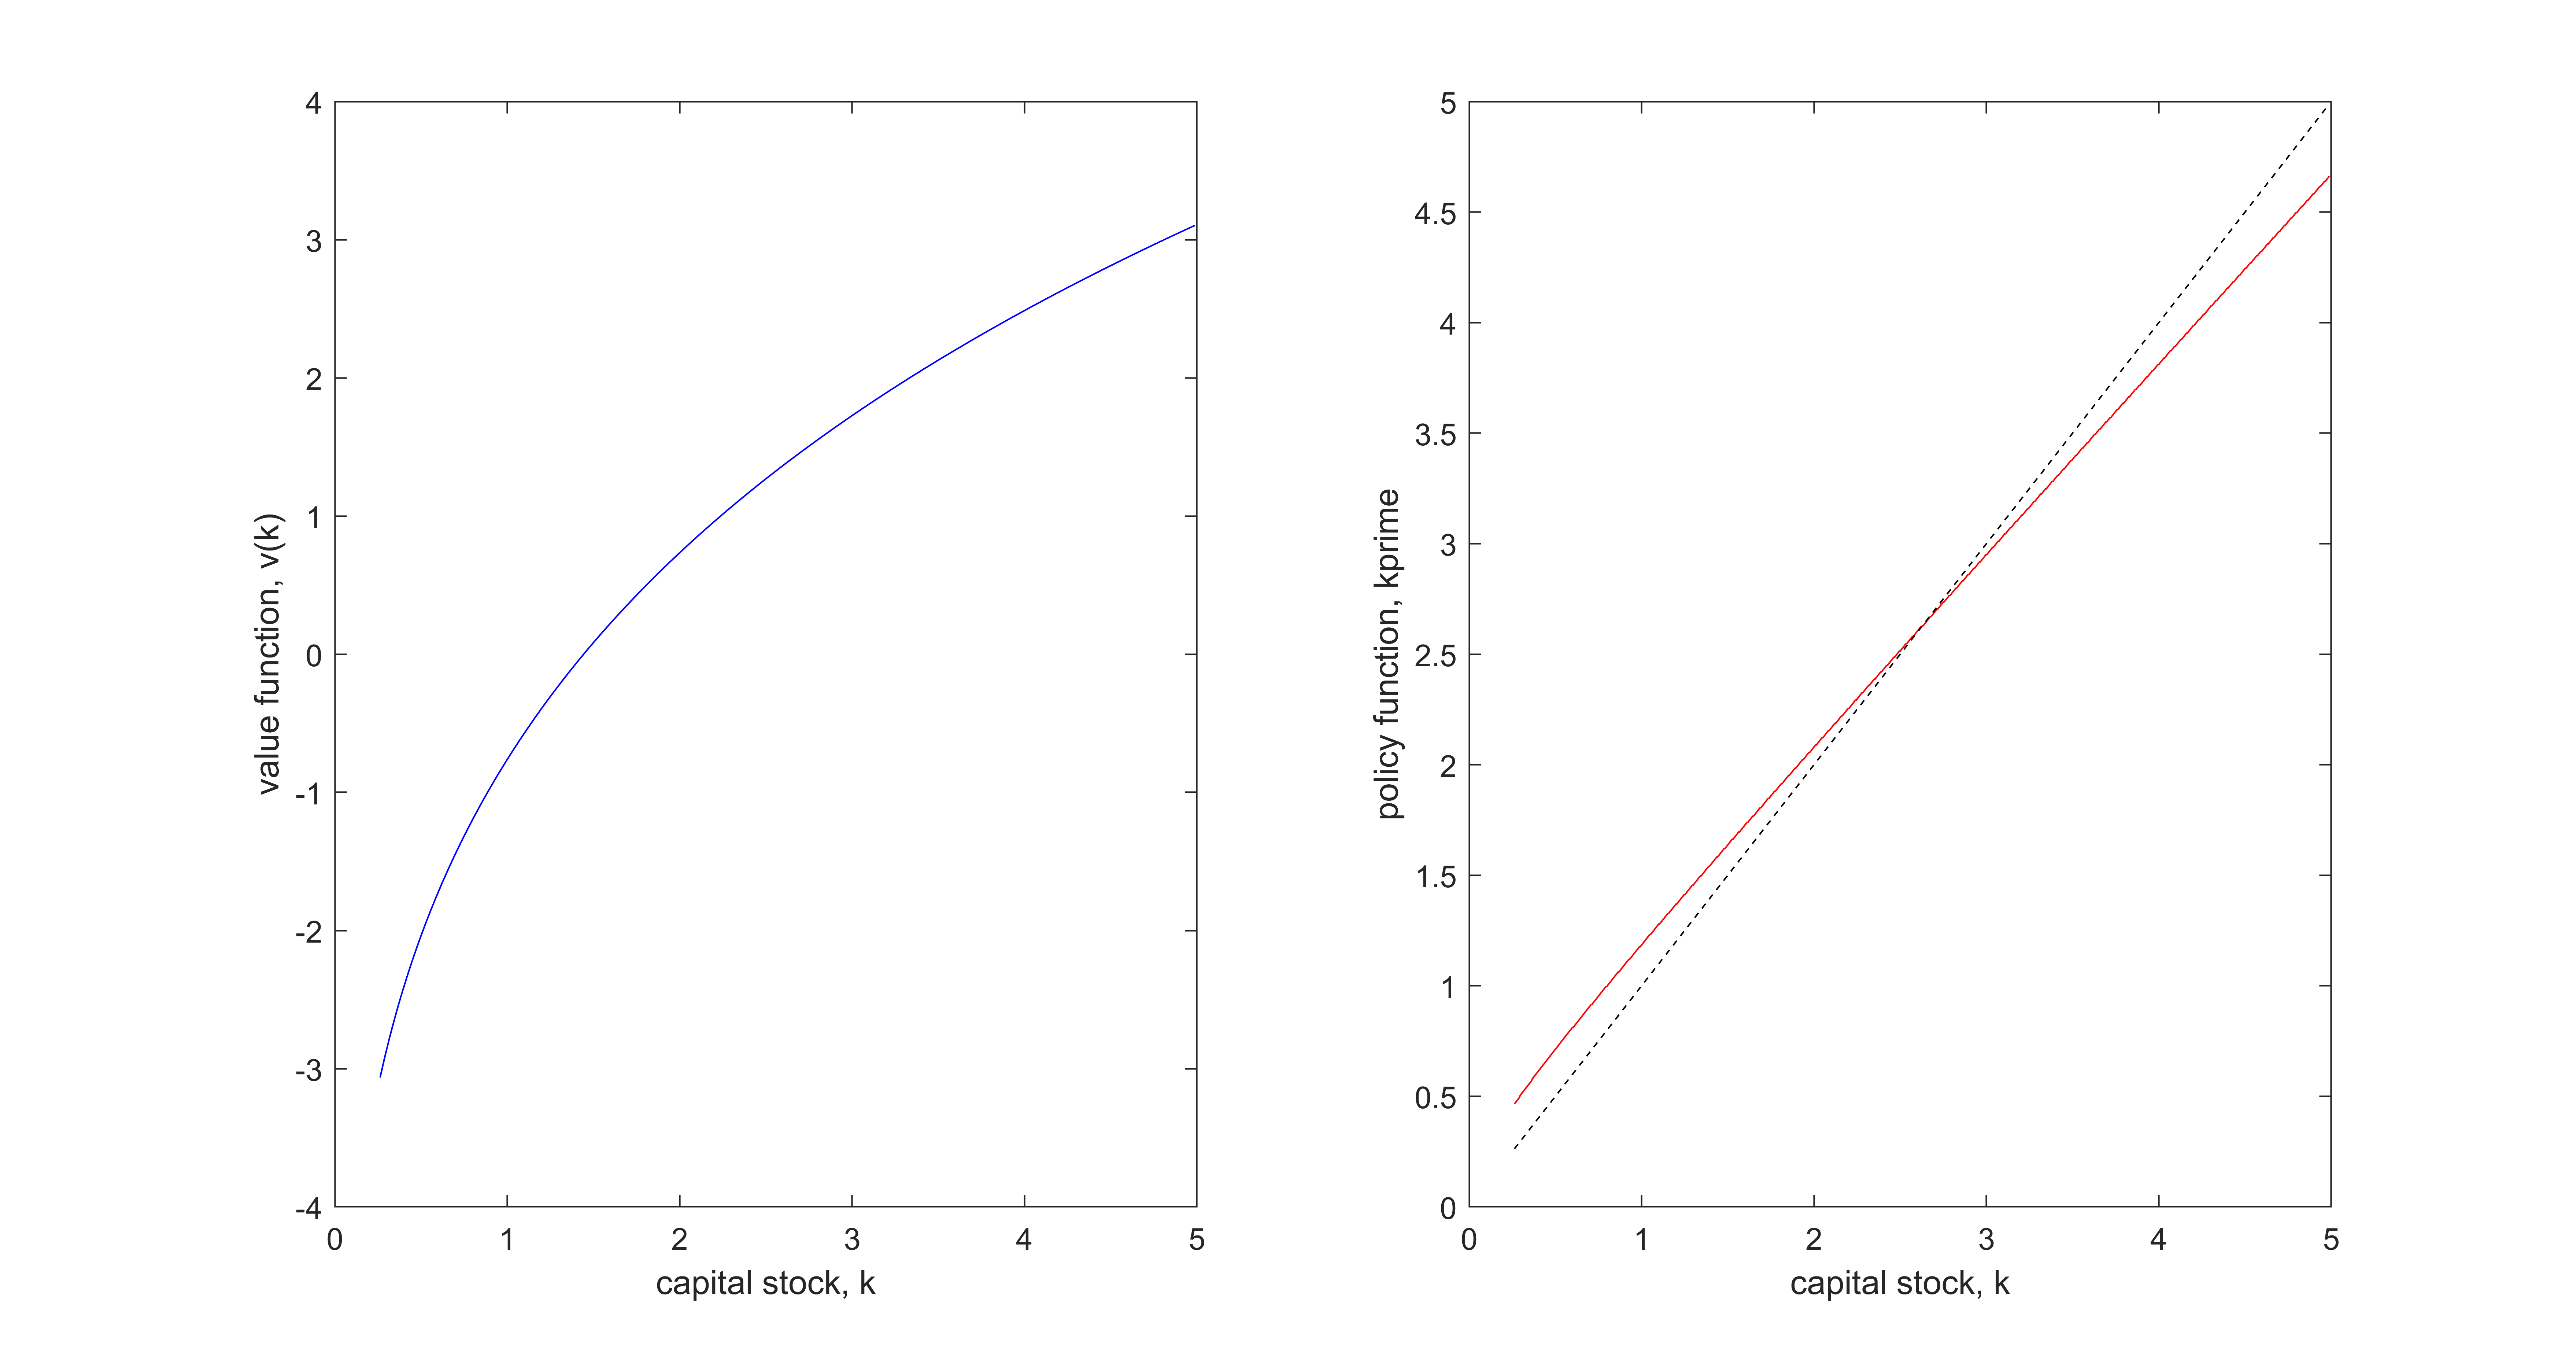
\includegraphics[width=1\textwidth]{figures/part1/ch2/fig-vfirck-value-policy-func.png}
    \caption{值函数与策略函数}
    \label{fig-vfirck-value-policy-func}
\end{figure}

% 2.6.2 ===== 改进VFI =====
\subsection{改进值函数迭代：插值}

上述方法的潜在问题之一是：\textbf{真实下期最优资本存量未必在我们设定的格点上}，
我们也就无法得到值函数在这些实际位置的取值。一个改进思路是利用插值法对值函数进行估计。
将状态变量格点取得相对宽松，而将控制变量格点取得较为精细，这样可减少对函数的估计次数，从而降低运算时间。
对如下形式的贝尔曼方程：
\begin{equation*}
    v(x) = \max_{y\in\mathbb{D}(x)} u(y,x) + \beta v(x^{\prime})
\end{equation*}
改进算法如下：

\begin{mdframed}[linecolor=Black,linewidth=1pt]
    \textbf{算法：改进值函数迭代}

    \textbf{输入：}模型参数（折现率、折旧率、风险偏好等）；算法参数（格点维数、停止准则等）

    \textbf{输出：}值函数$v$和策略函数$g$

    \textbf{1. 离散化状态变量和控制变量：}

    将状态变量$x$的取值空间离散化为较宽松的$N$个格点：
    \begin{equation*}
        \mathbb{X} = \{x_1<x_2<\cdots<x_i<\cdots<x_N\}
    \end{equation*}
    将控制变量$y$的取值空间离散化为较为精细的$M$个格点：
    \begin{equation*}
        \mathbb{Y} = \{y_1<y_2<\cdots<y_i<\cdots<y_M\}, ~ M \gg N
    \end{equation*}
    设定迭代次数$iter=0$，猜测初始值函数向量$v^0(x)$
    \begin{equation*}
        \left[v^0(x_1),v^0(x_2),\cdots,v^0(x_i),\cdots,v^0(x_N)\right]^{\prime}
    \end{equation*}
    选择停止准则$\varepsilon>0$

    \textbf{2. 求解贝尔曼方程右侧：}

    对任意$x_{i}\in\mathbb{X},~ i=1,\cdots,x_N$，根据运动方程计算下期状态：
    \begin{equation*}
        x^{\prime}_{ij} = h(y_j,x_i), ~\forall j=1,\cdots,M
    \end{equation*}
    \textbf{利用插值方法计算值函数在$x^{\prime}_{ij}=h(y_j,x_l)$处，当前迭代下的值函数取值}$\tilde{v}^{iter}(x^{\prime}_{ij})$，
    据此求解贝尔曼方程右侧：
    \begin{equation*}
        v^{iter+1}(x_i) \equiv v^{iter+1}_i = \max_{y\in\mathbb{Y}} u\left(y,x_i\right)
            + \beta \tilde{v}^{iter}(x^{\prime}_{ij})
    \end{equation*}

    \textbf{3. 检验停止准则：}

    若$\left\|v^{iter+1}(x)-v^{iter}(x)\right\|<\varepsilon$，则进行停止迭代，输出值函数和策略函数；
    否则回到第2步。
\end{mdframed}

\begin{lstlisting}
    %% setup
    % economic parpam
    alpha = 0.3;
    sigma = 1.5;
    beta = 0.95;
    delta = 0.1;

    ks = ((1-beta*(1-delta)) / (alpha*beta))^(1/(alpha-1));
    csy	= 1-alpha*beta*delta/(1-beta*(1-delta));

    % numerical param
    nk = 20;
    nc = 1000;
    epsilon = 1e-6;
    dev = 0.9;

    % discretize k
    kmin = (1-dev)*ks;
    kmax = (1+dev)*ks;
    kgrid = linspace(kmin,kmax,nk)';

    % discretize c
    cmin = 0.01;
    cmax = kmax^alpha;
    cgrid = linspace(cmin,cmax,nc)';

    %% iteration on bellman operator
    % initialize
    error = 1;
    v = ((csy*kgrid.^alpha).^(1-sigma)-1)./(1-sigma);    % value function
    tv = zeros(nk,1);
    g = zeros(nk,1);   % decision rule: index
    u = (cgrid.^(1-sigma)-1) / (1-sigma);
    iter = 1;

    % iteration
    tic
    while error > epsilon
    for i = 1:nk
        % all possible kp when ki now: nc*1 dimension
        kp = kgrid(i).^alpha + (1-delta)*kgrid(i) - cgrid; 
        % interp one函数用于正在kp处插值：nc*1 dimension
        vinterpl = interp1(kgrid,v, kp, 'spline'); 
        
        % bellman operator
        [tv(i),g(i)] = max(u+beta*vinterpl);
    end
    error = max(abs(tv-v));
    v = tv;
    iter = iter + 1;
    end
    toc

    %% solution
    c = cgrid(g);
    % kprime = kgrid(g);
    kprime = kgrid.^alpha+(1-delta)*kgrid-c;
\end{lstlisting}

用时仅0.05秒。


% =====   =====
\subsection{值函数迭代的改进：}



% =====   =====
\subsection{投影法的初步实现：配置算法}



% =====   =====
\subsection{Euler Based Methods}






% 第3章 数值方法

%导言

\chapter{数值方法}  \label{ch-numerical-methods}

在对确定性最有增长模型数值解的学习中，我们窥见了两种处理思路：
一是基于值函数（或策略函数）迭代的思路；另一是基于函数逼近直接处理值函数（或策略函数）的思路。
确定性最优增长模型结构简单，并且状态变量维度很低，只有资本存量$k$，两种方法都可以快速得到其数值解。
但是，量化宏观模型状态变量的维度通常较高，可能包含多个外生冲击或内生状态变量，部分异质性个体模型可能还涉及无穷维的分布作为状态，
这些都会带来维度诅咒（Curse of Dimention），导致基础的值函数迭代方法消耗大量计算时间，甚至不收敛等问题；
同时，对于较为复杂的模型，基础的函数逼近方法也面临可靠性下降的风险。
因此，必须对数值方法进行更进一步的学习，来解决这些麻烦。

本章将从随机最优增长模型开始，引出模型中计算条件期望的难点，并在马尔可夫假设下引出AR(1)过程的离散化方法，以解决这一难题；
其次，我们将介绍更为灵活和一般化的数值积分方法来处理期望的问题；
然后，我们将跳出值函数迭代的思想，直接从值函数入手解决问题：先介绍函数逼近方法，在此基础上着重研究投影方法的理论和应用；
最后，将对其他常用算法进行介绍。


% =============== main ch3 ===============

\input{parts/part1/p1c3/p1c31-eg-opt-growth.tex}
\input{parts/part1/p1c3/p1c32-markov.tex}
\input{parts/part1/p1c3/p1c33-discrete-approximation.tex}
\input{parts/part1/p1c3/p1c34-numerical-integeration.tex}
\input{parts/part1/p1c3/p1c35-func-approximation.tex}
\input{parts/part1/p1c3/p1c36-projection.tex}
\input{parts/part1/p1c3/p1c37-egm.tex}
% 第4章 完备市场理论

% 导言

\chapter{完备市场理论与宏观经济学中的均衡}  \label{ch-equilibrium}

目前为止，我们都是从\textbf{计划者}（Social Planner）角度和\textbf{代表性家庭}（同质家庭）的假设下处理最优增长模型。
在计划者问题中，计划者能够直接配置资源而不需要通过市场调节，因此价格并没有显示出现在优化问题中。
那么，计划者问题中的均衡能通过\textbf{市场配置}或者说\textbf{价格机制}实现吗？
即：如果经济是分散的（Decentralized Economy），存在家庭和企业等在市场上的互动，如何定义经济中的均衡，价格在其中起到什么作用？
这一（竞争）均衡产生的配置有什么特征，和计划者问题中的均衡配置有什么关系？
前一章动态规划和递归的框架能在定义均衡中起到什么作用？
代表性家庭的设定又为什么具有合理性？

回答上述问题离不开宏观经济学中的一个重要理论：完备市场（Complete Market）理论。
首先，本章将介绍完备市场理论中两种基础市场结构：\textbf{阿罗-德布鲁市场}和\textbf{序贯市场}；
其次，研究这两种市场下的竞争均衡与计划者问题（帕累托问题）均衡的关系；
同时，我们将指出这两种均衡定义方式的不足，并应用递归的思想定义递归竞争均衡；
再次，应用完备市场理论讨代表性家庭的存在性和资本资产定价问题；
最后，将相关均衡概念应用于一个分散经济下的最优增长模型，通过具体例子深入分析。


% =============== main ch4 ===============


% 4.1 ===== consumption saving =====
% 4.1 =============== Complete Market ===============

\section{完备市场理论基础}  \label{sec-complete-market}


% 4.1.1 ===== 经济环境设定（LS / Edmond / JLao）=====
\subsection{经济环境设定}

经济的时间是离散且无穷的：$t=0,1,\cdots, \infty$。在每一期，都有一个\textbf{随机事件}（Stochastic Event）实现，记为：
$$s_t\in S$$
通常我们将其称之为\textbf{状态}（State）。集合$S$是所有可能发生的事件的集合。记截至$t$时刻，所有实现事件的\textbf{历史}（History）为：
$$s^t = \left(s_0,s_1,\cdots,s_t\right) = \left(s^{t-1},s_t\right)$$
历史$s^t$发生的\textbf{无条件概率}（Unconditional Probability）记为：
$$\pi_t\left(s^t\right)$$
对时刻$t>\tau$，记在$s^{\tau}$实现的条件下，观测到$s^t$实现的\textbf{条件概率}（Conditional Probability）为：
$$\pi_t\left(s^t|s^{\tau}\right)$$
在本章，我们始终假设交易在观测到$s_0$的实现后进行，也就是说：$\pi_0\left(s_0\right)=1$。此外，我们暂时无需假设马尔可夫性。

经济中有$I$个个体（消费者），标记为$i=1,\cdots, I$。个体$i$获得的随机禀赋为$y_t^i\left(s^t\right)$，这一禀赋依赖于实现的事件历史$s^t$，
同时历史$s^t$是公共可观测的。个体$i$选择历史依赖的消费计划（History-Dependent Consumption Plan）：
$$
c^i \equiv \{c_t^i\left(s^t\right)\}_{t=0}^{\infty}
$$
个体（消费者）$i$的偏好为：
\begin{equation}    \label{eq-cm-preference-i}
    \begin{aligned}
        U_i\left(c^i\right) &\equiv \sum_{t=0}^{\infty} \sum_{s^t} \beta^t u_i\left(c_t^i\left(s^t\right)\right) \pi_t\left(s^t\right) \\
            &= \mathbb{E}_0 \sum_{t=0}^{\infty} \beta^t u_i\left(c_t^i\right)
    \end{aligned}
\end{equation}
其中，$\mathbb{E}_0$是基于$s_0$的\textbf{条件期望}。注意这里效用函数除了其自变量的下标不同，
我们同时允许不同个体效用函数本身结构的差异，即效用函数具有下标，即$u_i$，但所有个体的效用$u_i$都符合相关规范化假设，同时假设二次可微性。
此外，假设个体间分享概率$\pi_t\left(s^t\right)$的信息，即可以不使用记号$\pi_t^i$。
经济中的\textbf{可行配置}（Feasibale Allocation）满足资源约束：
\begin{equation}    \label{eq-cm-rc}
    \sum_i c_t^i\left(s^t\right) = \sum_i y_t^i\left(s^t\right), \quad \text { all } t, s^t
\end{equation}


% 4.1.2 ===== 两种交易结构（LS / Edmond / Kruger / PHS）=====
\subsection{两种交易结构}

\textbf{完备市场}是宏观经济学中的重要概念，它与\textbf{不完备市场}的主要区别在于：
经济中存在足够多的如状态依存合约等金融工具（数量覆盖未来所有可能的状态数），
个体通过交易这些工具构建资产组合，进而能够实现任意可行配置，对冲所有个体风险（Idiosyncratic Risk）。
\begin{definition}
    \textbf{状态依存合约}（State-Contingent Claims）是一种支付依赖于未来某个事件（状态）$s^t$是否实现的合约。
    例如如果未来可能发生$\{\text{晴天，下雨}\}$两种状态，消费者可以购买下雨时获得1单位消费品和晴天时获得1单位消费品的合约。
\end{definition}

完备市场可以在如下两种经典的市场结构下实现，我们在此分别介绍。

（1）\textbf{阿罗-德布鲁市场}（Arrow-Debreu Market） 

在Arrow-Debreu结构下，市场只在$t=0$时刻开放，
消费者在市场上交易的是对所有未来时刻$t\geq 1$的消费品的索取权（Complete Set of Contingent Consumption Claims）。
这些索取权是状态依存的（State-Contingent Claims）——依赖于截至$t$时所有可能发生的事件历史$s^t$，也被称为阿罗-德布鲁证券（Arrow-Debreu Security）。
在$t=0$时刻后，签订的合约生效，但没有额外交易再发生，因此这一交易结构也被称为\textbf{零时交易}（Time-Zero Trading）。
在阿罗-德布鲁市场中，由于能交易所有未来时间和可能状态下的消费品索取权（工具足够多），因此阿罗-德布鲁市场天然满足完备市场的定义。
\begin{property}
    阿罗-德布鲁市场天然是完备的。
\end{property}

（2）\textbf{序贯市场}（Sequential Market）

与Arrow-Debreu市场不同，序贯市场中的交易是按期进行的。市场每一期都会重新开放，但是市场上只存在一种
单期状态依存合约（one-period-ahead state-contingent claims）。
在$t$时刻，交易的范围仅针对已实现的历史$s^t$这一条件下所有可能的$s^{t+1}=\left(s^t,s_{t+1}\right)$。
序贯市场也被称为\textbf{阿罗市场}（Arrow Market）或Radner市场，其中的单期状态依存合约被称为\textbf{阿罗证券}（Arrow Securities）。
同样，如果每期都存在足够多的阿罗证券，可以覆盖下期所有可能状态，那么序贯市场也可以达到完备。但是，如果交易工具不足，则序贯交易可能无法达成完备性。
例如我们在后面不完备市场理论中将会看到的，若经济中仅存在单期无风险债券，则市场是不完备的。

\begin{property}
    序贯市场可以达到动态完备（Sequentially Complete）。但如果市场中只存在无风险债券，那么序贯市场是不完备的。
\end{property}

\cref{gr-admarket-tree}和\cref{gr-sqmarket-tree}分别给出了三期情形下一个两状态马尔科夫链在两种市场下的商品空间的例子。
随机事件$s_t\in S=\{0,1\}$。在阿罗-德布鲁市场下（\cref{gr-admarket-tree}），站在$t=0$时刻，$s_0=1$给定，截至$t=3$时刻所有可能的事件历史有8种。
个体在$t=0$时对$t\geq3$时所有8个可能节点下的商品索取权进行交易。
\cref{gr-sqmarket-tree}是在序贯市场下，截至$t=2$时刻实现的一个特定历史，和给定这一实现的历史下，$t=3$时刻的两种可能性。
在$t=2$，个体仅能交易在当前历史$(0,0,1)$下所能达到的$t=3$时节点的商品。

\begin{figure}
    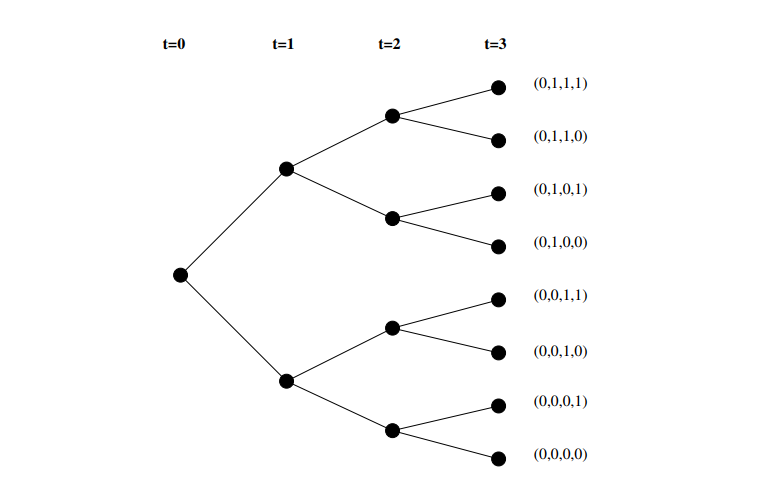
\includegraphics[width=1\textwidth]{figures/part1/ch4/admarket-tree.png}
    \caption{两状态马尔科夫链的阿罗-德布鲁商品空间}
    \label{gr-admarket-tree}
\end{figure}
\begin{figure}
    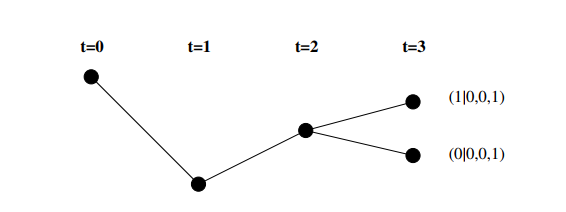
\includegraphics[width=1\textwidth]{figures/part1/ch4/sqmarket-tree.png}
    \caption{两状态马尔科夫链的阿罗-德布鲁商品空间}
    \label{gr-sqmarket-tree}
\end{figure}

两种市场结构对比而言，阿罗-德布鲁市场更近似一个理论基准，而序贯交易相对更贴近于现实市场。
此外，对于上述两种市场结构，我们很自然的会想到如下问题：
\begin{itemize}
    \item \textbf{两种市场中的均衡配置相同吗，与计划者均衡配置有什么关系？}
    \item \textbf{消费者的最优配置是否依赖于历史（History-Dependent）？}
\end{itemize}

我们将证明：两种市场交易结构会带来相同的帕累托最优配置，并且在完备市场下，$t$时刻的最优消费配置仅依赖部分刻画$t=0$时刻财富分布的时不变参数
和$t$时刻经济所实现的总禀赋，不会依赖带来相应总禀赋的历史。


% 4.1.3 ===== 计划者问题（Pareto Problem）=====
\subsection{帕累托问题}

在研究上述两种市场均衡配置的特征前，我们希望先定义一个基准配置用于进行比较，一个自然的想法是帕累托最优。
帕累托最优是指，无法使一个个体变得更好而同时不使其他个体变得更差。如果一个配置是帕累托最优的，我们称其为有效（efficient）。
我们可以通过为计划者解如下\textbf{帕累托问题}（Pareto Problem）找到一个有效配置。

计划者为每个个体$i=1,\cdots,I$选择$c^i \equiv \{c_t^i\left(s^t\right)\}_{t=0}^{\infty}$来最大化如下目标：
\begin{equation}    \label{eq-pareto-maxU}
    W=\sum_{i=1}^I \lambda_i U_i\left(c^i\right)
\end{equation}
其面临的资源约束为：
\begin{equation}    \label{eq-pareto-rc}
    \sum_i c_t^i\left(s^t\right) = \sum_i y_t^i\left(s^t\right) \quad \forall t, s^t
\end{equation}
其中$\lambda_i$是非负的\textbf{帕累托权重}（Pareto Weights）。
如果一个配置能构成一组非负权重下\textbf{上述问题的解}，我们就称这一配置为\textbf{帕累托有效}（Pareto Efficient）。
对这一优化问题，构建拉格朗日函数：
\begin{equation*}
    \begin{aligned}
        \mathcal{L} &= \sum_i \lambda_i \sum_{t=0}^{\infty} \sum_{s^t} \beta^t u_i\left(c_t^i\left(s^t\right)\right) \pi_t\left(s^t\right)
                    + \sum_{t=0}^{\infty} \sum_{s^t} \theta_t\left(s^t\right) \sum_i\left[y_t^i\left(s^t\right)-c_t^i\left(s^t\right)\right] \\
                    &= \sum_{t=0}^{\infty} \sum_{s^t}
                    \left\{\sum_{i=1}^I \lambda_i \beta^t u_i\left(c_t^i\left(s^t\right)\right) \pi_t\left(s^t\right)
                        +\theta_t\left(s^t\right) \sum_{i=1}^I\left[y_t^i\left(s^t\right)-c_t^i\left(s^t\right)\right]\right\} \\
                    &= \sum_i \sum_{t=0}^{\infty} \sum_{s^t}
                    \left\{\lambda_i \beta^t u_i\left(c_t^i\left(s^t\right)\right) \pi_t\left(s^t\right)
                        +\theta_t\left(s^t\right)\left[y_t^i\left(s^t\right)-c_t^i\left(s^t\right)\right]\right\}
    \end{aligned}
\end{equation*}
其中非负的$\theta_t\left(s^t\right)$为第$t$期和历史$s^t$对应约束的拉格朗日乘子。
从这一优化问题的形式上看，计划者实际面临的是一个静态问题（Static Problem）序列，因为问题中并不涉及跨期变量。
具体看，对$c_t^i\left(s^t\right)$求解FOC得：
\begin{equation}    \label{eq-pareto-foc}
    \lambda_i \beta^t u_i^{\prime}\left(c_t^i\left(s^t\right)\right) \pi_t\left(s^t\right)=\theta_t\left(s^t\right) \quad \forall i, t, s^t
\end{equation}
不失一般性，取个体$i$和个体$1$，将他们的FOC结合可得：
\begin{equation}    \label{eq-pareto-r-foc}
    \frac{u_i^{\prime}\left(c_t^i\left(s^t\right)\right)}{u_1^{\prime}\left(c_t^1\left(s^t\right)\right)}=\frac{\lambda_1}{\lambda_i}
        \quad \forall t, s^t
\end{equation}
也即：
\begin{equation}    \label{eq-pareto-ci}
    c_t^i\left(s^t\right)=u_i^{\prime-1}\left(\frac{\lambda_1}{\lambda_i} u_1^{\prime}\left(c_t^1\left(s^t\right)\right)\right)
\end{equation}
这意味着任意个体的消费都可以写为关于个体1的消费$c_t^1\left(s^t\right)$的函数。进一步，将上式代入资源约束\ref{eq-cm-rc}可得：
\begin{equation}    \label{eq-pareto-c1}
    \sum_i u_i^{\prime-1}\left(\frac{\lambda_1}{\lambda_i} u_1^{\prime}\left(c_t^1\left(s^t\right)\right)\right)
        =\sum_i y_t^i\left(s^t\right) \equiv Y_t\left(s^t\right) \quad \forall t, s^t
\end{equation}
注意到，式\ref{eq-pareto-c1}是关于$c_1^t\left(s^t\right)$的单一非线性方程（Single Nonlinear Equation）。
右侧对$i$的求和可以定义为经济的\textbf{总禀赋}，而由于帕累托权重$\{\lambda_i\}_{i=1}^I$是一组给定的参数，因此左侧对$i$求和后也与个体$i$无关，
进而可以从中解出$c_t^1\left(s^t\right)$。

进一步观察式\ref{eq-pareto-c1}可知，给定一组外生参数$\{\lambda_i\}_{i=1}^I$，$c_t^1\left(s^t\right)$\textbf{只依赖当前实现的总禀赋}，
既不依赖时刻$t$，也不依赖特定的能够带来当前总禀赋的历史$s^t$或是在$t$时刻个体禀赋的分布。
同时，式\ref{eq-pareto-ci}将$c_t^i$表为了$c_t^1\left(s^t\right)$的函数，从而可得其余所有个体的消费配置$c_t^i\left(s^t\right)$：
同样是只依赖于所实现的总禀赋的。至此，我们就得到了计划者在参数$\{\lambda_i\}_{i=1}^I$下的一个帕累托有效配置，且均衡解的形式是一个时不变函数：
\begin{equation*}
    c_t^i\left(s^t\right) = f\left(\lambda_i, Y_t ; \boldsymbol{\lambda}\right)
\end{equation*}

\begin{property}
    对于计划者的帕累托问题，一组\textbf{有效配置}具有如下特征：
    \begin{itemize}
        \item 与时间$t$无关，与历史无关（\textit{history-independent or history-free}）：当前的$Y_t$是所有历史的充分统计量；
        \item 与$t$时刻个体禀赋的分布无关（\textit{distribution-free}）：只有求和后的$Y_t$重要。
    \end{itemize}
\end{property}
假设存在两条不同历史路径$s^t$和$\tilde{s}^{\tau}$，但只要$Y_t\left(s^t\right)=Y_{\tau}\left(\tilde{s}^{\tau}\right)$，
就有$c_t^i\left(s^t\right)=c_{\tau}^i\left(\tilde{s}^\tau\right)$。

进一步观察\ref{eq-pareto-r-foc}式，对任意两个个体$(i,j)$成立：
\begin{equation*}
    \frac{u_i^{\prime}\left(c_t^i\left(s^t\right)\right)}{u_j^{\prime}\left(c_t^1\left(s^t\right)\right)}=\frac{\lambda_j}{\lambda_i}
        \quad \forall t, s^t
\end{equation*}
也就是说，\textbf{在任何有效配置中，个体间消费边际效用比在任意时刻、任意历史下都相等}。
背后的经济含义是:计划者通过维持不同个体间消费边际效用比来为所有个体在任意时间和状态下提供\textbf{消费保险（Consumption Insurance）}。
由于计划者问题中除了总的资源约束外不存在其他约束，因此很自然的将这一情形定义为\textbf{完美消费保险}（Perfect Consumption Insurance）或
\textbf{完美风险承担}（Perfect Risk Sharing）。

\begin{definition}  \label{def-perfect-c-insurance}
    \textbf{完美消费保险}（Perfect Consumption Insurance），或称\textbf{完美风险承担}（Perfect Risk Sharing），
    是指一组消费配置$\{c^i=\{c_t^i\left(s^t\right)\}_{t=0}^{\infty}\}_{i=1}^{I}$：
    使不同个体间的消费边际效用比在任意时刻、任意状态下都相同（Constant across any time and states）。
\end{definition}

至此，我们通过求解计划者的帕累托问题，建立了一个基准均衡配置。这一均衡是\textbf{帕累托有效}的，因为计划者不可能使某一个体变好而不使其他人变差。
从计算的角度看：我们通过式\ref{eq-pareto-c1}解出$c_t^1\left(s^t\right)$，
再通过式\ref{eq-pareto-ci}解出其余个体的$c_t^i\left(s^t\right)$。并且由式\ref{eq-pareto-ci}可知：
只有不同个体间帕累托权重的比值是值得关注的。因此，我们可以进行正则化，将权重和定为1：$\sum_{i}\lambda_i = 1$。
由于每个个体的消费配置只是总禀赋的函数，因此其个体消费与总禀赋（总消费）完全相关，并且所占份额与其所分配得的帕累托权重相关。



% 4.2 ===== consumption saving =====
\input{parts/part1/p1c4/p1c4-2-ra-existence.tex}


% 4.3 ===== consumption saving =====
% 4.3 =============== CAPM ===============

\section{资本资产定价（CAPM）}  \label{sec-capm}




% 4.4 ===== consumption saving =====
\input{parts/part1/p1c4/p1c4-4-decentralized-equlibrium.tex}


% 第5章 DSGE

% 导言

\chapter{DSGE}  \label{ch-dsge}





% =============== main ch5 ===============

% 5.1 =============== RBC ===============

\section{RBC}   \label{sec-rbc}
% 5.2 ===============  Solve by Linearization ===============

\section{Linearization} \label{linearization}

% 5.3 =============== NK-DSGE ===============

\section{新凯恩斯-DSGE} \label{sec-nk-dsge}

% =============== 第6章 宏观计量 ==============

% 导言




\chapter{宏观计量理论与方法}    \label{ch-macro-econometrics}



% =============== main ch6 ===============

\input{parts/part1/p1c6/p1c61-empirical-macro-methods.tex}
\input{parts/part1/p1c6/p1c62-dsge-estimate-bayes.tex}
\input{parts/part1/p1c6/p1c63-structure-estimate.tex}



% 第二篇：量化核心理论
\part{量化宏观核心理论}

% =============== 第7章 不完全市场理论 ==============

% 导言


\chapter{不完全市场理论}    \label{ch-incomplete-market}



% =============== main ch7 ===============

% 7.1 =============== PE下的不完全市场 ===============

\section{局部均衡下的不完全市场} \label{sec-pe-incomplete}


% 7.2 =============== PE下的不完全市场 ===============

\section{一般均衡下的不完全市场} \label{sec-ge-incomplete}




% =============== 第8章 总体不确定下的异质性模型 ===============

% 导言


\chapter{总体不确定下的异质性模型}    \label{ch-ha-agg-uncertainty}


% =============== main ch8 ===============

% 8.1 =============== KS模型 ===============

\section{Krusell-Smith算法} \label{sec-ks}


% 8.2 =============== 复制KS ===============

\section{实现KS算法} \label{sec-replicate-ks}


% 8.3 =============== Reiter ===============

\section{Reiter算法} \label{sec-reiter}



% =============== 第9章 企业动态模型 ===============

% 导言


\chapter{企业动态}    \label{ch-firm-dynamics}


% =============== main ch8 ===============

% 9.1 =============== 企业动态模型 ===============

\section{企业动态基础} \label{sec-basic-firm-dynamics}


% 9.2 =============== 企业动态模型 ===============

\section{微观异质性与宏观动态} \label{sec-micro-hetero-macro-dynamics}






% 第三篇：HANK模型
\part{现代量化宏观主要模型：HANK}

% =============== 第10章 异质性家庭 ==============

% 导言


\chapter{异质性家庭理论}    \label{ch-house-hetero}



% =============== main ch10 ===============

% 10.1 =============== TANK ===============

\section{TANK模型} \label{sec-tank}


% 10.1 =============== HANK ===============

\section{HANK模型} \label{sec-hank}



% =============== 第11章 异质性企业 ==============

% 导言


\chapter{异质性企业理论}    \label{ch-firm-hetero}



% =============== main ch10 ===============

% 11.1 =============== Solve firm hetero ===============

\section{异质性企业模型求解} \label{sec-solve-firm-hetero}


% 11.2 =============== 金融异质性 ===============

\section{金融异质性} \label{sec-financial-hetero}





% 第四篇：量化专题
\part{量化宏观专题}

% =============== 第12章 宏观债务、周期与政策 ==============

% 导言


\chapter{宏观债务、周期与政策}    \label{ch-macro-debt-policy}



% =============== main ch10 ===============

% 12.1 =============== firm debt ===============

\section{企业债务} \label{sec-firm-debt}


% 12.2 =============== house debt ===============

\section{家庭债务} \label{sec-house-debt}


% 12.3 =============== gov debt ===============

\section{政府债务} \label{sec-gov-debt}



% =============== 第13章 银行、金融危机与宏观政策 ==============

% 导言


\chapter{银行、金融危机与宏观政策}    \label{ch-bank-crisis-policy}



% =============== main ch10 ===============

% 13.1 =============== 银行挤兑 ===============

\section{银行挤兑} \label{sec-bank-run}

% 13.2 =============== 银行资本 ===============

\section{银行资本} \label{sec-bank-capital}

% 13.3 =============== 宏观政策管理 ===============

\section{宏观政策与金融危机} \label{sec-crisis-macro-policy}


% =============== 第14章 宏观债务、周期与政策 ==============

% 导言


\chapter{异质性模型前沿理论}    \label{ch-computation-hetero}



% =============== main ch14 ===============

% 14.1 =============== 结构方法 ===============

\section{Structural Method} \label{sec-structural-method}

% 14.2 =============== AI ===============

\section{深度强化学习与分布计算} \label{sec-deep-reinforcement-learning}




% ===== 后辅文 =====
\appendix

\include{back/appendix}

\backmatter

%\bibliographystyle{apalike}
%\bibliography{back/refs}

\printbibliography[title={参考文献}]

\end{document}